
\documentclass{article} % For LaTeX2e
\usepackage{iclr2026_conference,times}
\usepackage{graphicx} 
\usepackage{booktabs}
\usepackage{subcaption}
\usepackage{todonotes}
\usepackage{pgfmath}
% Optional math commands from https://github.com/goodfeli/dlbook_notation.
%%%%% NEW MATH DEFINITIONS %%%%%

\usepackage{amsmath,amsfonts,bm}

% Mark sections of captions for referring to divisions of figures
\newcommand{\figleft}{{\em (Left)}}
\newcommand{\figcenter}{{\em (Center)}}
\newcommand{\figright}{{\em (Right)}}
\newcommand{\figtop}{{\em (Top)}}
\newcommand{\figbottom}{{\em (Bottom)}}
\newcommand{\captiona}{{\em (a)}}
\newcommand{\captionb}{{\em (b)}}
\newcommand{\captionc}{{\em (c)}}
\newcommand{\captiond}{{\em (d)}}

% Highlight a newly defined term
\newcommand{\newterm}[1]{{\bf #1}}


% Figure reference, lower-case.
\def\figref#1{figure~\ref{#1}}
% Figure reference, capital. For start of sentence
\def\Figref#1{Figure~\ref{#1}}
\def\twofigref#1#2{figures \ref{#1} and \ref{#2}}
\def\quadfigref#1#2#3#4{figures \ref{#1}, \ref{#2}, \ref{#3} and \ref{#4}}
% Section reference, lower-case.
\def\secref#1{section~\ref{#1}}
% Section reference, capital.
\def\Secref#1{Section~\ref{#1}}
% Reference to two sections.
\def\twosecrefs#1#2{sections \ref{#1} and \ref{#2}}
% Reference to three sections.
\def\secrefs#1#2#3{sections \ref{#1}, \ref{#2} and \ref{#3}}
% Reference to an equation, lower-case.
\def\eqref#1{equation~\ref{#1}}
% Reference to an equation, upper case
\def\Eqref#1{Equation~\ref{#1}}
% A raw reference to an equation---avoid using if possible
\def\plaineqref#1{\ref{#1}}
% Reference to a chapter, lower-case.
\def\chapref#1{chapter~\ref{#1}}
% Reference to an equation, upper case.
\def\Chapref#1{Chapter~\ref{#1}}
% Reference to a range of chapters
\def\rangechapref#1#2{chapters\ref{#1}--\ref{#2}}
% Reference to an algorithm, lower-case.
\def\algref#1{algorithm~\ref{#1}}
% Reference to an algorithm, upper case.
\def\Algref#1{Algorithm~\ref{#1}}
\def\twoalgref#1#2{algorithms \ref{#1} and \ref{#2}}
\def\Twoalgref#1#2{Algorithms \ref{#1} and \ref{#2}}
% Reference to a part, lower case
\def\partref#1{part~\ref{#1}}
% Reference to a part, upper case
\def\Partref#1{Part~\ref{#1}}
\def\twopartref#1#2{parts \ref{#1} and \ref{#2}}

\def\ceil#1{\lceil #1 \rceil}
\def\floor#1{\lfloor #1 \rfloor}
\def\1{\bm{1}}
\newcommand{\train}{\mathcal{D}}
\newcommand{\valid}{\mathcal{D_{\mathrm{valid}}}}
\newcommand{\test}{\mathcal{D_{\mathrm{test}}}}

\def\eps{{\epsilon}}


% Random variables
\def\reta{{\textnormal{$\eta$}}}
\def\ra{{\textnormal{a}}}
\def\rb{{\textnormal{b}}}
\def\rc{{\textnormal{c}}}
\def\rd{{\textnormal{d}}}
\def\re{{\textnormal{e}}}
\def\rf{{\textnormal{f}}}
\def\rg{{\textnormal{g}}}
\def\rh{{\textnormal{h}}}
\def\ri{{\textnormal{i}}}
\def\rj{{\textnormal{j}}}
\def\rk{{\textnormal{k}}}
\def\rl{{\textnormal{l}}}
% rm is already a command, just don't name any random variables m
\def\rn{{\textnormal{n}}}
\def\ro{{\textnormal{o}}}
\def\rp{{\textnormal{p}}}
\def\rq{{\textnormal{q}}}
\def\rr{{\textnormal{r}}}
\def\rs{{\textnormal{s}}}
\def\rt{{\textnormal{t}}}
\def\ru{{\textnormal{u}}}
\def\rv{{\textnormal{v}}}
\def\rw{{\textnormal{w}}}
\def\rx{{\textnormal{x}}}
\def\ry{{\textnormal{y}}}
\def\rz{{\textnormal{z}}}

% Random vectors
\def\rvepsilon{{\mathbf{\epsilon}}}
\def\rvtheta{{\mathbf{\theta}}}
\def\rva{{\mathbf{a}}}
\def\rvb{{\mathbf{b}}}
\def\rvc{{\mathbf{c}}}
\def\rvd{{\mathbf{d}}}
\def\rve{{\mathbf{e}}}
\def\rvf{{\mathbf{f}}}
\def\rvg{{\mathbf{g}}}
\def\rvh{{\mathbf{h}}}
\def\rvu{{\mathbf{i}}}
\def\rvj{{\mathbf{j}}}
\def\rvk{{\mathbf{k}}}
\def\rvl{{\mathbf{l}}}
\def\rvm{{\mathbf{m}}}
\def\rvn{{\mathbf{n}}}
\def\rvo{{\mathbf{o}}}
\def\rvp{{\mathbf{p}}}
\def\rvq{{\mathbf{q}}}
\def\rvr{{\mathbf{r}}}
\def\rvs{{\mathbf{s}}}
\def\rvt{{\mathbf{t}}}
\def\rvu{{\mathbf{u}}}
\def\rvv{{\mathbf{v}}}
\def\rvw{{\mathbf{w}}}
\def\rvx{{\mathbf{x}}}
\def\rvy{{\mathbf{y}}}
\def\rvz{{\mathbf{z}}}

% Elements of random vectors
\def\erva{{\textnormal{a}}}
\def\ervb{{\textnormal{b}}}
\def\ervc{{\textnormal{c}}}
\def\ervd{{\textnormal{d}}}
\def\erve{{\textnormal{e}}}
\def\ervf{{\textnormal{f}}}
\def\ervg{{\textnormal{g}}}
\def\ervh{{\textnormal{h}}}
\def\ervi{{\textnormal{i}}}
\def\ervj{{\textnormal{j}}}
\def\ervk{{\textnormal{k}}}
\def\ervl{{\textnormal{l}}}
\def\ervm{{\textnormal{m}}}
\def\ervn{{\textnormal{n}}}
\def\ervo{{\textnormal{o}}}
\def\ervp{{\textnormal{p}}}
\def\ervq{{\textnormal{q}}}
\def\ervr{{\textnormal{r}}}
\def\ervs{{\textnormal{s}}}
\def\ervt{{\textnormal{t}}}
\def\ervu{{\textnormal{u}}}
\def\ervv{{\textnormal{v}}}
\def\ervw{{\textnormal{w}}}
\def\ervx{{\textnormal{x}}}
\def\ervy{{\textnormal{y}}}
\def\ervz{{\textnormal{z}}}

% Random matrices
\def\rmA{{\mathbf{A}}}
\def\rmB{{\mathbf{B}}}
\def\rmC{{\mathbf{C}}}
\def\rmD{{\mathbf{D}}}
\def\rmE{{\mathbf{E}}}
\def\rmF{{\mathbf{F}}}
\def\rmG{{\mathbf{G}}}
\def\rmH{{\mathbf{H}}}
\def\rmI{{\mathbf{I}}}
\def\rmJ{{\mathbf{J}}}
\def\rmK{{\mathbf{K}}}
\def\rmL{{\mathbf{L}}}
\def\rmM{{\mathbf{M}}}
\def\rmN{{\mathbf{N}}}
\def\rmO{{\mathbf{O}}}
\def\rmP{{\mathbf{P}}}
\def\rmQ{{\mathbf{Q}}}
\def\rmR{{\mathbf{R}}}
\def\rmS{{\mathbf{S}}}
\def\rmT{{\mathbf{T}}}
\def\rmU{{\mathbf{U}}}
\def\rmV{{\mathbf{V}}}
\def\rmW{{\mathbf{W}}}
\def\rmX{{\mathbf{X}}}
\def\rmY{{\mathbf{Y}}}
\def\rmZ{{\mathbf{Z}}}

% Elements of random matrices
\def\ermA{{\textnormal{A}}}
\def\ermB{{\textnormal{B}}}
\def\ermC{{\textnormal{C}}}
\def\ermD{{\textnormal{D}}}
\def\ermE{{\textnormal{E}}}
\def\ermF{{\textnormal{F}}}
\def\ermG{{\textnormal{G}}}
\def\ermH{{\textnormal{H}}}
\def\ermI{{\textnormal{I}}}
\def\ermJ{{\textnormal{J}}}
\def\ermK{{\textnormal{K}}}
\def\ermL{{\textnormal{L}}}
\def\ermM{{\textnormal{M}}}
\def\ermN{{\textnormal{N}}}
\def\ermO{{\textnormal{O}}}
\def\ermP{{\textnormal{P}}}
\def\ermQ{{\textnormal{Q}}}
\def\ermR{{\textnormal{R}}}
\def\ermS{{\textnormal{S}}}
\def\ermT{{\textnormal{T}}}
\def\ermU{{\textnormal{U}}}
\def\ermV{{\textnormal{V}}}
\def\ermW{{\textnormal{W}}}
\def\ermX{{\textnormal{X}}}
\def\ermY{{\textnormal{Y}}}
\def\ermZ{{\textnormal{Z}}}

% Vectors
\def\vzero{{\bm{0}}}
\def\vone{{\bm{1}}}
\def\vmu{{\bm{\mu}}}
\def\vtheta{{\bm{\theta}}}
\def\va{{\bm{a}}}
\def\vb{{\bm{b}}}
\def\vc{{\bm{c}}}
\def\vd{{\bm{d}}}
\def\ve{{\bm{e}}}
\def\vf{{\bm{f}}}
\def\vg{{\bm{g}}}
\def\vh{{\bm{h}}}
\def\vi{{\bm{i}}}
\def\vj{{\bm{j}}}
\def\vk{{\bm{k}}}
\def\vl{{\bm{l}}}
\def\vm{{\bm{m}}}
\def\vn{{\bm{n}}}
\def\vo{{\bm{o}}}
\def\vp{{\bm{p}}}
\def\vq{{\bm{q}}}
\def\vr{{\bm{r}}}
\def\vs{{\bm{s}}}
\def\vt{{\bm{t}}}
\def\vu{{\bm{u}}}
\def\vv{{\bm{v}}}
\def\vw{{\bm{w}}}
\def\vx{{\bm{x}}}
\def\vy{{\bm{y}}}
\def\vz{{\bm{z}}}

% Elements of vectors
\def\evalpha{{\alpha}}
\def\evbeta{{\beta}}
\def\evepsilon{{\epsilon}}
\def\evlambda{{\lambda}}
\def\evomega{{\omega}}
\def\evmu{{\mu}}
\def\evpsi{{\psi}}
\def\evsigma{{\sigma}}
\def\evtheta{{\theta}}
\def\eva{{a}}
\def\evb{{b}}
\def\evc{{c}}
\def\evd{{d}}
\def\eve{{e}}
\def\evf{{f}}
\def\evg{{g}}
\def\evh{{h}}
\def\evi{{i}}
\def\evj{{j}}
\def\evk{{k}}
\def\evl{{l}}
\def\evm{{m}}
\def\evn{{n}}
\def\evo{{o}}
\def\evp{{p}}
\def\evq{{q}}
\def\evr{{r}}
\def\evs{{s}}
\def\evt{{t}}
\def\evu{{u}}
\def\evv{{v}}
\def\evw{{w}}
\def\evx{{x}}
\def\evy{{y}}
\def\evz{{z}}

% Matrix
\def\mA{{\bm{A}}}
\def\mB{{\bm{B}}}
\def\mC{{\bm{C}}}
\def\mD{{\bm{D}}}
\def\mE{{\bm{E}}}
\def\mF{{\bm{F}}}
\def\mG{{\bm{G}}}
\def\mH{{\bm{H}}}
\def\mI{{\bm{I}}}
\def\mJ{{\bm{J}}}
\def\mK{{\bm{K}}}
\def\mL{{\bm{L}}}
\def\mM{{\bm{M}}}
\def\mN{{\bm{N}}}
\def\mO{{\bm{O}}}
\def\mP{{\bm{P}}}
\def\mQ{{\bm{Q}}}
\def\mR{{\bm{R}}}
\def\mS{{\bm{S}}}
\def\mT{{\bm{T}}}
\def\mU{{\bm{U}}}
\def\mV{{\bm{V}}}
\def\mW{{\bm{W}}}
\def\mX{{\bm{X}}}
\def\mY{{\bm{Y}}}
\def\mZ{{\bm{Z}}}
\def\mBeta{{\bm{\beta}}}
\def\mPhi{{\bm{\Phi}}}
\def\mLambda{{\bm{\Lambda}}}
\def\mSigma{{\bm{\Sigma}}}

% Tensor
\DeclareMathAlphabet{\mathsfit}{\encodingdefault}{\sfdefault}{m}{sl}
\SetMathAlphabet{\mathsfit}{bold}{\encodingdefault}{\sfdefault}{bx}{n}
\newcommand{\tens}[1]{\bm{\mathsfit{#1}}}
\def\tA{{\tens{A}}}
\def\tB{{\tens{B}}}
\def\tC{{\tens{C}}}
\def\tD{{\tens{D}}}
\def\tE{{\tens{E}}}
\def\tF{{\tens{F}}}
\def\tG{{\tens{G}}}
\def\tH{{\tens{H}}}
\def\tI{{\tens{I}}}
\def\tJ{{\tens{J}}}
\def\tK{{\tens{K}}}
\def\tL{{\tens{L}}}
\def\tM{{\tens{M}}}
\def\tN{{\tens{N}}}
\def\tO{{\tens{O}}}
\def\tP{{\tens{P}}}
\def\tQ{{\tens{Q}}}
\def\tR{{\tens{R}}}
\def\tS{{\tens{S}}}
\def\tT{{\tens{T}}}
\def\tU{{\tens{U}}}
\def\tV{{\tens{V}}}
\def\tW{{\tens{W}}}
\def\tX{{\tens{X}}}
\def\tY{{\tens{Y}}}
\def\tZ{{\tens{Z}}}


% Graph
\def\gA{{\mathcal{A}}}
\def\gB{{\mathcal{B}}}
\def\gC{{\mathcal{C}}}
\def\gD{{\mathcal{D}}}
\def\gE{{\mathcal{E}}}
\def\gF{{\mathcal{F}}}
\def\gG{{\mathcal{G}}}
\def\gH{{\mathcal{H}}}
\def\gI{{\mathcal{I}}}
\def\gJ{{\mathcal{J}}}
\def\gK{{\mathcal{K}}}
\def\gL{{\mathcal{L}}}
\def\gM{{\mathcal{M}}}
\def\gN{{\mathcal{N}}}
\def\gO{{\mathcal{O}}}
\def\gP{{\mathcal{P}}}
\def\gQ{{\mathcal{Q}}}
\def\gR{{\mathcal{R}}}
\def\gS{{\mathcal{S}}}
\def\gT{{\mathcal{T}}}
\def\gU{{\mathcal{U}}}
\def\gV{{\mathcal{V}}}
\def\gW{{\mathcal{W}}}
\def\gX{{\mathcal{X}}}
\def\gY{{\mathcal{Y}}}
\def\gZ{{\mathcal{Z}}}

% Sets
\def\sA{{\mathbb{A}}}
\def\sB{{\mathbb{B}}}
\def\sC{{\mathbb{C}}}
\def\sD{{\mathbb{D}}}
% Don't use a set called E, because this would be the same as our symbol
% for expectation.
\def\sF{{\mathbb{F}}}
\def\sG{{\mathbb{G}}}
\def\sH{{\mathbb{H}}}
\def\sI{{\mathbb{I}}}
\def\sJ{{\mathbb{J}}}
\def\sK{{\mathbb{K}}}
\def\sL{{\mathbb{L}}}
\def\sM{{\mathbb{M}}}
\def\sN{{\mathbb{N}}}
\def\sO{{\mathbb{O}}}
\def\sP{{\mathbb{P}}}
\def\sQ{{\mathbb{Q}}}
\def\sR{{\mathbb{R}}}
\def\sS{{\mathbb{S}}}
\def\sT{{\mathbb{T}}}
\def\sU{{\mathbb{U}}}
\def\sV{{\mathbb{V}}}
\def\sW{{\mathbb{W}}}
\def\sX{{\mathbb{X}}}
\def\sY{{\mathbb{Y}}}
\def\sZ{{\mathbb{Z}}}

% Entries of a matrix
\def\emLambda{{\Lambda}}
\def\emA{{A}}
\def\emB{{B}}
\def\emC{{C}}
\def\emD{{D}}
\def\emE{{E}}
\def\emF{{F}}
\def\emG{{G}}
\def\emH{{H}}
\def\emI{{I}}
\def\emJ{{J}}
\def\emK{{K}}
\def\emL{{L}}
\def\emM{{M}}
\def\emN{{N}}
\def\emO{{O}}
\def\emP{{P}}
\def\emQ{{Q}}
\def\emR{{R}}
\def\emS{{S}}
\def\emT{{T}}
\def\emU{{U}}
\def\emV{{V}}
\def\emW{{W}}
\def\emX{{X}}
\def\emY{{Y}}
\def\emZ{{Z}}
\def\emSigma{{\Sigma}}

% entries of a tensor
% Same font as tensor, without \bm wrapper
\newcommand{\etens}[1]{\mathsfit{#1}}
\def\etLambda{{\etens{\Lambda}}}
\def\etA{{\etens{A}}}
\def\etB{{\etens{B}}}
\def\etC{{\etens{C}}}
\def\etD{{\etens{D}}}
\def\etE{{\etens{E}}}
\def\etF{{\etens{F}}}
\def\etG{{\etens{G}}}
\def\etH{{\etens{H}}}
\def\etI{{\etens{I}}}
\def\etJ{{\etens{J}}}
\def\etK{{\etens{K}}}
\def\etL{{\etens{L}}}
\def\etM{{\etens{M}}}
\def\etN{{\etens{N}}}
\def\etO{{\etens{O}}}
\def\etP{{\etens{P}}}
\def\etQ{{\etens{Q}}}
\def\etR{{\etens{R}}}
\def\etS{{\etens{S}}}
\def\etT{{\etens{T}}}
\def\etU{{\etens{U}}}
\def\etV{{\etens{V}}}
\def\etW{{\etens{W}}}
\def\etX{{\etens{X}}}
\def\etY{{\etens{Y}}}
\def\etZ{{\etens{Z}}}

% The true underlying data generating distribution
\newcommand{\pdata}{p_{\rm{data}}}
% The empirical distribution defined by the training set
\newcommand{\ptrain}{\hat{p}_{\rm{data}}}
\newcommand{\Ptrain}{\hat{P}_{\rm{data}}}
% The model distribution
\newcommand{\pmodel}{p_{\rm{model}}}
\newcommand{\Pmodel}{P_{\rm{model}}}
\newcommand{\ptildemodel}{\tilde{p}_{\rm{model}}}
% Stochastic autoencoder distributions
\newcommand{\pencode}{p_{\rm{encoder}}}
\newcommand{\pdecode}{p_{\rm{decoder}}}
\newcommand{\precons}{p_{\rm{reconstruct}}}

\newcommand{\laplace}{\mathrm{Laplace}} % Laplace distribution

\newcommand{\E}{\mathbb{E}}
\newcommand{\Ls}{\mathcal{L}}
\newcommand{\R}{\mathbb{R}}
\newcommand{\emp}{\tilde{p}}
\newcommand{\lr}{\alpha}
\newcommand{\reg}{\lambda}
\newcommand{\rect}{\mathrm{rectifier}}
\newcommand{\softmax}{\mathrm{softmax}}
\newcommand{\sigmoid}{\sigma}
\newcommand{\softplus}{\zeta}
\newcommand{\KL}{D_{\mathrm{KL}}}
\newcommand{\Var}{\mathrm{Var}}
\newcommand{\standarderror}{\mathrm{SE}}
\newcommand{\Cov}{\mathrm{Cov}}
% Wolfram Mathworld says $L^2$ is for function spaces and $\ell^2$ is for vectors
% But then they seem to use $L^2$ for vectors throughout the site, and so does
% wikipedia.
\newcommand{\normlzero}{L^0}
\newcommand{\normlone}{L^1}
\newcommand{\normltwo}{L^2}
\newcommand{\normlp}{L^p}
\newcommand{\normmax}{L^\infty}

\newcommand{\parents}{Pa} % See usage in notation.tex. Chosen to match Daphne's book.

\DeclareMathOperator*{\argmax}{arg\,max}
\DeclareMathOperator*{\argmin}{arg\,min}

\DeclareMathOperator{\sign}{sign}
\DeclareMathOperator{\Tr}{Tr}
\let\ab\allowbreak


\usepackage{hyperref}
\usepackage{url}
\usepackage{wrapfig}
\usepackage{subcaption}
\usepackage{amsthm}
\usepackage[table]{xcolor}
\usepackage{multirow} 

\newtheorem{proposition}{Proposition}
\newtheorem{lemma}{Lemma}
\newtheorem{theorem}{Theorem}
\theoremstyle{remark}
\newtheorem{remark}{Remark}
\newtheorem{assumption}{Assumption}
\newtheorem{corollary}{Corollary}



\definecolor{frappe_rosewater}{RGB}{242, 213, 207}
\definecolor{frappe_flamingo}{RGB}{238, 190, 190}
\definecolor{frappe_pink}{RGB}{244, 184, 228}
\definecolor{frappe_mauve}{RGB}{202, 158, 230}
\definecolor{frappe_red}{RGB}{231, 130, 132}
\definecolor{frappe_maroon}{RGB}{234, 153, 156}
\definecolor{frappe_peach}{RGB}{239, 159, 118}
\definecolor{frappe_yellow}{RGB}{229, 200, 144}
\definecolor{frappe_green}{RGB}{166, 209, 137}
\definecolor{frappegreen}{RGB}{166, 209, 137}
\definecolor{frappe_teal}{RGB}{129, 200, 190}
\definecolor{frappe_sky}{RGB}{153, 209, 219}
\definecolor{frappe_sapphire}{RGB}{133, 193, 220}
\definecolor{frappe_blue}{RGB}{140, 170, 238}
\definecolor{frappe_lavender}{RGB}{186, 187, 241}

\definecolor{latte_rosewater}{RGB}{220, 138, 120}
\definecolor{latte_flamingo}{RGB}{221, 120, 120}
\definecolor{latte_pink}{RGB}{234, 118, 203}
\definecolor{latte_mauve}{RGB}{136, 57, 239}
\definecolor{latte_red}{RGB}{210, 15, 57}
\definecolor{latte_maroon}{RGB}{230, 69, 83}
\definecolor{latte_peach}{RGB}{254, 100, 11}
\definecolor{latte_yellow}{RGB}{223, 142, 29}
\definecolor{latte_green}{RGB}{64, 160, 43}
\definecolor{latte_teal}{RGB}{23, 146, 153}
\definecolor{latte_sky}{RGB}{4, 165, 229}
\definecolor{latte_sapphire}{RGB}{32, 159, 181}
\definecolor{latte_blue}{RGB}{30, 102, 245}
\definecolor{latte_lavender}{RGB}{114, 135, 253}
\newcommand{\colorcell}[3]{%
  \pgfmathsetmacro{\intensity}{round(100*(#1-#2)/(#3-#2))}
  \cellcolor{frappegreen!\intensity}
}

\setuptodonotes{inline, color=frappe_red}


\title{\textsc{LIFT-CF}: Lifting Counterfactual \\ Explanations to Distributional Robustness}

% Authors must not appear in the submitted version. They should be hidden
% as long as the \iclrfinalcopy macro remains commented out below.
% Non-anonymous submissions will be rejected without review.

\author{Antiquus S.~Hippocampus, Natalia Cerebro \& Amelie P. Amygdale \thanks{ Use footnote for providing further information
about author (webpage, alternative address)---\emph{not} for acknowledging
funding agencies.  Funding acknowledgements go at the end of the paper.} \\
Department of Computer Science\\
Cranberry-Lemon University\\
Pittsburgh, PA 15213, USA \\
\texttt{\{hippo,brain,jen\}@cs.cranberry-lemon.edu} \\
\And
Ji Q. Ren \& Yevgeny LeNet \\
Department of Computational Neuroscience \\
University of the Witwatersrand \\
Joburg, South Africa \\
\texttt{\{robot,net\}@wits.ac.za} \\
\AND
Coauthor \\
Affiliation \\
Address \\
\texttt{email}
}

% The \author macro works with any number of authors. There are two commands
% used to separate the names and addresses of multiple authors: \And and \AND.
%
% Using \And between authors leaves it to \LaTeX{} to determine where to break
% the lines. Using \AND forces a linebreak at that point. So, if \LaTeX{}
% puts 3 of 4 authors names on the first line, and the last on the second
% line, try using \AND instead of \And before the third author name.

\newcommand{\fix}{\marginpar{FIX}}
\newcommand{\new}{\marginpar{NEW}}

%\iclrfinalcopy % Uncomment for camera-ready version, but NOT for submission.
\begin{document}


\maketitle

\begin{abstract}
Counterfactual explanations (CFs) recommend actionable changes an individual can make to flip a machine learning model's prediction toward a desired outcome. 
Most CF generators assume a static model and data distribution, yet models deployed in practice are retrained periodically, so a CF that is valid today may not be tomorrow. 
Institutions that deploy these models typically issue a population of CFs, so  robustness is fundamentally a population-level property, not an individual-level one.
Existing robustness methods, however, certify or optimize validity of each CF individually, leaving this population-level risk unaddressed.
We introduce \textsc{LIFT-CF}, a distributionally robust wrapper that treats the population of CFs produced by any CF generator as the object to be made robust, rather than any single CF. 
\textsc{LIFT-CF} constructs a Wasserstein ambiguity set anchored to both the observed target-class distribution and the generator's own CF output, and shows that minimizing a tractable upper bound on the worst-case risk over this set reduces to moving the CF distribution along a calibrated Wasserstein barycentric path. \textcolor{latte_maroon}{Extensive experiments across ... show that ...}
\end{abstract}

\section{Introduction}
\begin{wrapfigure}[18]{r}{0.45\textwidth}
\vspace{-2em}
  \begin{center}
    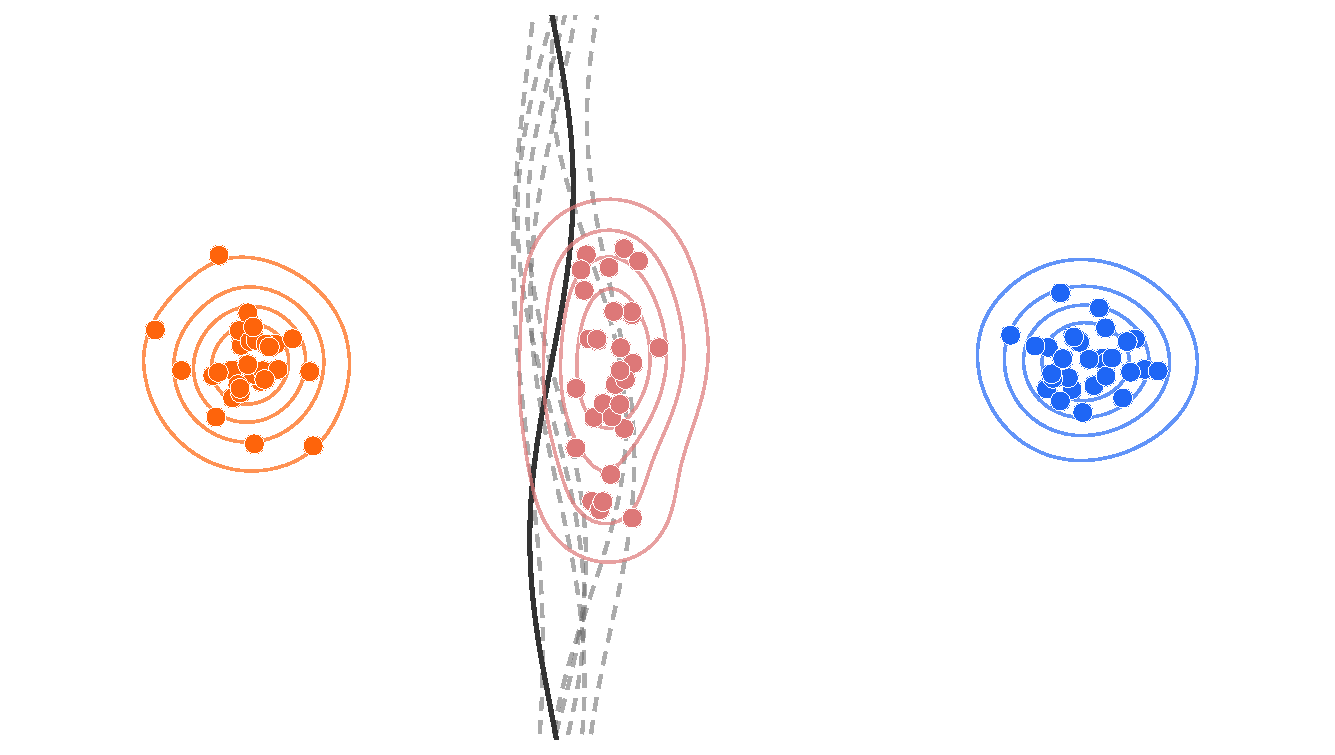
\includegraphics[trim={1.5cm 2cm 1.5cm 2cm},clip,width=\linewidth]{Figures/cf_sketch_proximal.pdf}
  \end{center}
  \caption{\textbf{Illustrative example of decision boundary shift.} A population of counterfactuals (pink) sits near a decision boundary (solid curve) separating two class distributions (orange and blue). Dashed lines indicate how the boundary's position could shift, illustrating why a counterfactual valid under the current boundary may become invalid under a shifted one.}
    \label{fig:robustness}
\end{wrapfigure}


Counterfactual explanations (CFs) help users identify changes that would alter a machine learning model's prediction. 
During the generation process, most methods assume a fixed model and data distribution; in deployment, however, the setting is considerably more dynamic~\citep{quionero2009dataset}. 
Evolving data distributions or policy changes cause retraining, and previously generated CFs might lose their validity in the new setting~\citep{rawal2020algorithmic}.
A counterfactual explanation that recommends actions to alter a model's prediction is only useful if the action still delivers the desired outcome for a model that might have been updated in between. 
When it does not, the recourse for a user, for example, an applicant told to raise their income by \$ 3000 to secure loan  approval, expires, undermining the trustworthiness and utility of CFs in dynamic environments (Figure~\ref{fig:robustness}).



This concern is not only at an individual level but also distributional. 
A bank, for instance, does not provide a single counterfactual but a population of them, one per rejected applicant. When the underlying data distribution shifts and the model is retrained, it is not only one CF but a fraction of the previously generated population that becomes invalid.
From an institutional perspective, the relevant object of robustness is not the individual CF but the distributional risk of invalidity across the entire generated population, a risk that instance-by-instance certification cannot control, since it never represents the population as an object of its own.





Current strategies aim to ensure that a counterfactual remains valid despite model updates. 
One line of work constrains these changes \emph{implicitly}, without directly modeling how the model might change: counterfactuals are optimized for high classification certainty~\citep{dutta2022robust,Hamman2023Robust, DBLP:conf/aaai/JiangL0T23}, training data is augmented with CFs~\citep{ferrario2022robustness}, or robustness is certified a posteriori under a Bayesian view over a user-specified pool of retrained models~\citep{stkepka2025counterfactual, duell2026provably}. 
Another line of work models the changes \emph{explicitly}, bounding against plausible parameter shifts for a single CF~\cite{upadhyay2021towards,kayastha2024learning,kyaw2025optimal, Marzari2024Rigorous,DBLP:conf/acml/JiangLL0T23}, including against a mixture of plausible future parameter distributions~\citep{DBLP:conf/iclr/NguyenBN23}. 
Two works come closer to a population view: \citet{bui2022counterfactual} jointly optimize a small per-instance set of CFs for joint validity under a shifted model, while \citet{nguyen2022robust} perturb the data distribution directly but still certify recourse one input at a time.
Neither treats the population generated across instances as the object of robustness.

% \begin{wrapfigure}[30]{r}{0.5\textwidth}
% \vspace{-2em}
%     \centering
%     \begin{subfigure}[b]{0.32\textwidth}
%         \centering
%         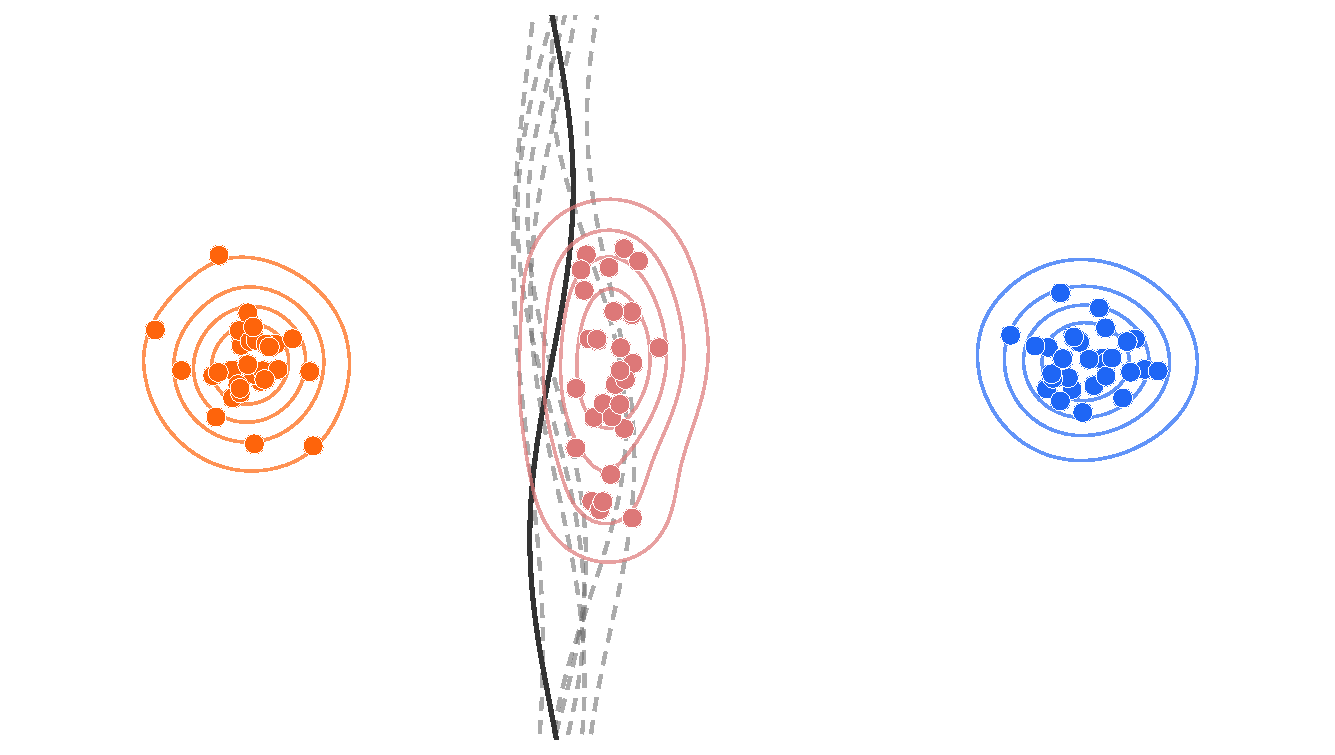
\includegraphics[trim={1.5cm 2cm 1.5cm 2cm},clip,width=\linewidth]{Figures/cf_sketch_proximal.pdf}
%         \caption{Proximal CFs.}
%         \label{fig:proximal}
%     \end{subfigure}
    
%     \vspace{4pt}
    
%     \begin{subfigure}[b]{0.32\textwidth}
%         \centering
%         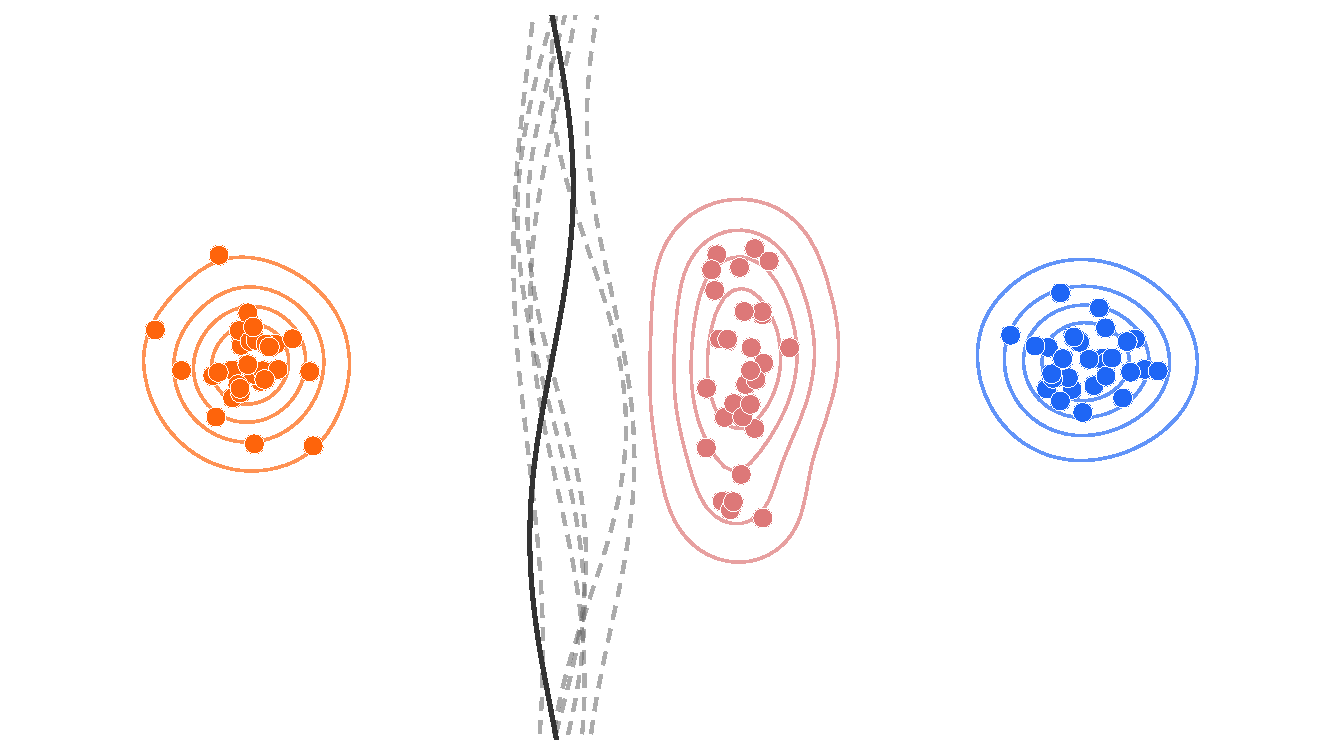
\includegraphics[trim={1.5cm 2cm 1.5cm 2cm},clip,width=\linewidth]{Figures/cf_sketch_robust.pdf}
%         \caption{Robust CFs.}
%         \label{fig:robust}
%     \end{subfigure}
    
%     \vspace{4pt}
    
%     \begin{subfigure}[b]{0.32\textwidth}
%         \centering
%         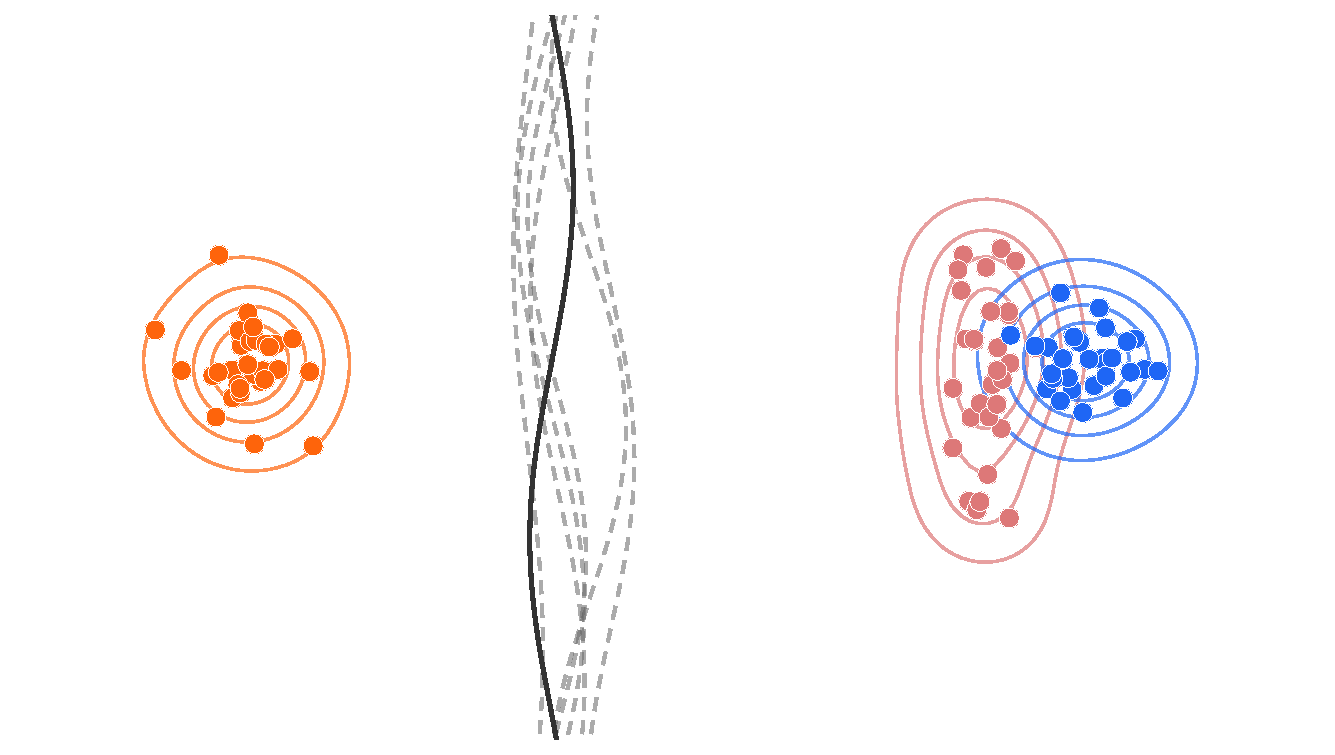
\includegraphics[trim={1.5cm 2cm 1.5cm 2cm},clip,width=\linewidth]{Figures/cf_sketch_plausible.pdf}
%         \caption{Plausible CFs.}
%         \label{fig:plausible}
%     \end{subfigure}
    
%     \caption{\textbf{Counterfactual types under decision boundary shift.} Counterfactuals (pink) are generated near a decision boundary (solid curve) separating two class distributions (orange and blue). Dashed lines show possible boundary shifts. \textbf{(a) Proximal} CFs stay close to the original boundary and become invalid under shift. \textbf{(c) Plausible} CFs lie within the target class distribution, by disregarding proximity, they often require larger and less actionable changes than necessary. \textbf{(b) Robust} CFs stay as close as possible to the original input, combining actionability of (a) with the robustness of (c). }
%     \label{fig:overall}
% \end{wrapfigure}

We address this gap with \textsc{LIFT-CF}, a post-hoc distributional refinement that treats the population of CFs produced by any CF generator as a distribution to be moved, via a calibrated Wasserstein lens anchored to the target class and the generator's output, toward a region of lower worst-case future invalidity.
Our main contributions are:
\begin{itemize}
    \item We introduce the \emph{CF-induced Wasserstein lens}, an ambiguity set of target-side distributions close to the observed target class and generator output, giving a worst-case notion of distributional lens risk that a refined CF population can be optimized against.
    \item We show that minimizing a tractable convex relaxation of this worst-case risk reduces to a one-dimensional Wasserstein barycentric family between the CF and target distributions, and select the deployed refinement by directly evaluating robustness to adversarial retraining shifts on held-out data, with a matching Lipschitz stability guarantee bounding the resulting finite-grid search error.
    \item We realize the calibrated refinement via optimal transport and show empirically that it \textcolor{latte_maroon}{experiments?}
\end{itemize}
\section{Related Work}\label{sec:related}

%\subsection{Data Shifts}
%Data shifts pose a fundamental challenge in machine learning, broadly categorized into \emph{covariate shift}, \emph{label shift}, and \emph{concept shift}, etc.~\cite{quionero2009dataset}. To systematically examine data shifts, we categorize them into two main types \cite{10.5555/3692070.3692237}:
%(i) Data Corruptions: alterations in the distribution’s support, i.e., changes in the observed data instances themselves, often arising from measurement errors, environmental disturbances, or adversarial manipulations. Examples include background noise affecting speech recognition systems~\cite{kinoshita2020deep}, numerical rounding errors in financial computations~\cite{li2015rounding}, adversarial modifications in image classification tasks~\cite{goodfellow2020explaining}, and distortions in decision-making processes caused by Goodhart’s law in public aid allocation~\cite{camacho2011goodhart};
%(ii) Subpopulation Shifts: changes to the distribution’s density or mass function while its support remains unchanged. Notable examples include demographic changes influencing recommendation systems~\cite{blodgett2016demographic,sapiezynski2017algorithmic}, temporal shifts affecting diagnostic accuracy in healthcare~\cite{pasterkamp2017moving}, and spatial distribution changes disrupting wildlife conservation models~\cite{beery2021iwildcam}. By proactively modeling these shifts within the training dataset, rather than reacting to them post-deployment, our method builds robustness into CF generation directly.

%\subsection{Robust CFs}

%Ensuring robustness under various perturbations remains a key research challenge. Prior work has explored robustness from multiple perspectives, including robustness against model changes, model multiplicity, noisy execution, and input variations. Among these, our work aligns most closely with robustness against model changes and model multiplicity. Therefore, we provide a more detailed discussion on them. For a comprehensive overview of other robustness methods, we refer readers to the relevant survey paper \cite{ijcai2024p894}.

%\subsubsection{Robustness against Model Changes}
Model parameter updates typically arise from retraining on new data~\cite{rawal2020algorithmic}. Existing approaches constrain such changes either \emph{implicitly}, without modeling their source, or \emph{explicitly}, by model plausible parameter shifts .

\textbf{Implicit constraints.}
The methods optimize CFs for high classification certainty~\cite{dutta2022robust,Hamman2023Robust,DBLP:conf/aaai/JiangL0T23}, augment training data with generated CFs~\cite{ferrario2022robustness}, or perturb the covariance of data sampled near the decision boundary to train a linear surrogate~\cite{DBLP:journals/ior/BuiNYN25}. \citet{xu2024generally} relax the naturally-occurring model change condition of \citet{Hamman2023Robust} to a subgaussian bound. Two works certify robustness a posteriori under a Bayesian view over a user-specified pool of retrained models: \citet{stkepka2025counterfactual} move a base CF into a region meeting a specified robustness level, while \citet{duell2026provably} optimize on the generation side for high confidence and low variance in the CF's posterior predictive distribution, certifying graceful degradation via a KL-divergence bound.


\textbf{Explicit constraints.}
\citet{upadhyay2021towards} introduce ROAR, %the notion of plausible model shifts and 
a minimax objective generating CFs that minimize the worst-case plausible shift under a linear surrogate %of the (possibly nonlinear) 
model; \citet{kayastha2024learning} give a provably optimal solver for any generalized linear model, and \citet{kyaw2025optimal} extend this to general $L_p$-bounded neighborhoods. \citet{DBLP:conf/iclr/NguyenBN23} similarly hedge against plausible parameter shifts via a min-max problem, where the max term is the Gelbrich distance to an ambiguity set of future model-parameter distributions, solved by gradient descent. \citet{bui2022counterfactual} instead bound the joint validity probability of a set of CFs. AP$\Delta$S~\cite{Marzari2024Rigorous,marzari2025probabilistically} samples plausible model shifts directly and shows exact robustness decisions are NP-hard. \citet{DBLP:conf/acml/JiangLL0T23,jiang2024interval} propagate interval-valued weights and biases through the network to bound hidden-unit activations under bounded parameter perturbations.
%A limitation shared by these explicit, parameter-space approaches is that they assume model changes stem from minor data shifts without modeling the data shift itself. 
These parameter-space approaches assume model changes stem from data shifts without modeling the shift itself.
\citet{nguyen2022robust} address this by adversarially perturbing the data via a Gaussian-mixture ambiguity set over Wasserstein distance on the mean-covariance space.
Two works come closest to a population view: \citet{bui2022counterfactual} jointly optimize a small per-instance CF set for joint validity, while \citet{nguyen2022robust}, despite modeling the data shift, still certifies recourse one input at a time. Neither treats the population of generated CFs as the robustness object, the gap our method closes.

A related line of work study robustness to \emph{model multiplicity}~\cite{breiman2001statistical,Marx2020Predictive,Black2022Selective,Rudin2019Stop,coston2021characterizing,pawelczyk2020counterfactual,turbal2026ellice}, where distinct near-optimal models yield inconsistent CFs, with no assumption on how or why models differ. See~\cite{ijcai2024p894} for a broader robustness survey.

%Most existing research on CF robustness focuses on ensuring validity under model parameter updates, which typically occur within the model's original structural framework. Such modifications arise when models are retrained on data from slightly altered distributions \cite{rawal2020algorithmic}, aligning with our study's framework. Recent works have explored various ways to define the boundaries of model changes. For instance, \cite{upadhyay2021towards} introduced the concept of plausible model variations, constraining parameter updates to perturbations within a predefined magnitude. Formally, given an input $x$, model $f$, and CF $x'$, their framework ensures that CFs remain valid under bounded parameter shifts, requiring both the original model ff and the perturbed model $f'$ to assign the same classification to $x'$. This fundamental idea has been extended in \cite{Black2022Consistent,Jiang2023Provably,Jiang2023Formalising,Marzari2024Rigorous}, all maintaining the core requirement that CFs remain consistent across model updates. In contrast, \cite{Hamman2023Robust} expanded the scope beyond artificially bounded perturbations, considering naturally occurring model shifts in neural networks. Their approach eliminates explicit magnitude constraints, allowing theoretically unbounded parameter changes while ensuring local consistency in model behavior near the explained input. While these methodologies vary in how they define acceptable model changes—some imposing strict constraints while others allowing greater flexibility—there is a shared recognition that model instability undermines the reliability of explanations. This issue is particularly evident in high-stakes scenarios, such as fluctuating loan approval outcomes across model updates. A key limitation of existing approaches is their assumption that model changes stem from small data shifts, yet they do not explicitly analyze these shifts in depth. Since future data distributions remain uncertain, accounting for such shifts makes the problem more complex. In contrast, our method takes a proactive approach by modeling and anticipating the most probable data shifts, ensuring greater robustness in CFs.





%Model multiplicity refers to the phenomenon where multiple distinct models achieve comparable predictive performance for the same task \cite{breiman2001statistical,Marx2020Predictive}. While one common approach aggregates predictions from these models into a unified output \cite{Black2022Selective}, recent studies indicate that such ensemble models may still exhibit inconsistent behavior — both in terms of predictions and their explanations — when applied to individual instances \cite{Rudin2019Stop,coston2021characterizing}. This inconsistency has significant implications for CFs: a CF generated for an aggregated prediction may not remain valid across all constituent models, potentially leading to contradictions and undermining user trust in explanation consistency. To address this, \cite{pawelczyk2020counterfactual} anchor explanations to a specific model's predictions and ensure CF validity across potential classifier updates, mirroring the goals of robustness against model changes. Unlike that line of work, model multiplicity does not assume updates are driven by shifts in data distribution, and places no constraints on the architecture or training methodology of either the base model generating CFs or the alternative models considered.

\section{Distributionally Robust Counterfactuals}

We propose \textsc{LIFT-CF}, a distributional robustness wrapper for CF generators that operates \emph{post-hoc} on the population of CFs a generator produces, rather than modifying its objective or parameters.
We first state the exact robustness objective and show it is intractable to optimize directly (Section~\ref{sec:objective}). 
%We start by defining the problem of distributionally robust counterfactuals and then describe how our new distributional robustness wrapper \textsc{LIFT-CF} operates \emph{post-hoc} on the population of CFs a generator produces.
We then construct a CF-induced Wasserstein lens, a tractable, data-level relaxation that captures where the CF distribution should lie to remain valid under future shifts, and show under an explicit regularity condition that it provably controls the exact objective (Section~\ref{sec:lens}). The robust relaxation of the resulting minimax objective induces a one-dimensional Wasserstein barycentric family (Section~\ref{sec:barycentric}), on which we select the deployed operating point by evaluating the true objective directly, using held-out proxy deployment shifts (Section~\ref{subsec:wro}). We show this one-dimensional objective is Lipschitz along the path and bound the resulting finite-grid search error (Section~\ref{sec:stability}).
Finally, we realize the selected refinement via optimal transport (Section~\ref{sec:transport}).

\subsection{Problem Setting and the Robust Objective}\label{sec:objective}
\iffalse
We study the refinement of a generated population of counterfactuals toward a region that remains robust to future shifts, while preserving the generator's original CF structure. A CF that is favorable under the current classifier does not necessarily remain favorable once the classifier is updated: a shift in the decision boundary may move the CF back into the unfavorable region. 
Since the future classifier is unobserved at deployment time, we cannot hedge against a single predicted shift. 
\fi

Let $f_0: \mathcal{X}\to[0,1]$ be a binary classifier and $\tau\in(0,1)$ a decision threshold; $x$ is \emph{favorable} if
$f_0(x)\ge\tau$ and \emph{unfavorable} otherwise. 
Write $\ell_f(z) = [\tau-f(z)]_+$ for the margin-based counterfactual invalidity loss. 
Let $G$ be a base CF generator. Given a batch $X=\{x_i\}_{i=1}^n$ of instances with $f_0(x_i)<\tau$, let $z_i = G(x_i)$ denote the corresponding CFs for a favorable outcome.
We represent the generated CF population by its empirical distribution
$
\mathbb{P}_{\mathrm{CF}} = \frac{1}{n}\sum_{i=1}^n \delta_{z_i},
$
and let $\mathbb{P}_1$ denote the empirical distribution of target-class training samples ($f_0(x)\ge\tau$).
The two distributions provide complementary information: $\mathbb{P}_{\mathrm{CF}}$ captures where the base generator currently places CFs, while $\mathbb{P}_1$ captures the observed structure of the favorable class. 
We use \textcolor{frappe_red}{consistency} to denote closeness to $\mathbb P_{\mathrm{CF}}$, and \emph{plausibility} to denote alignment with $\mathbb P_1$. 
%Note that $\mathbb P_{\mathrm{CF}}$ may resemble proximal CFs in the typical sense, i.e., close to the original instances, as we assume no prior knowledge about the base generator's internal objective.

A CF favorable under $f_0$ does not necessarily remain favorable once $f_0$ is updated: a shift in the decision boundary may move the CF back into the unfavorable region. 
Since the future classifier is unobserved at deployment time, we cannot hedge against a single predicted shift.
%\paragraph{The robust objective.}
%The initial classifier $f_0$ is not fixed over a CF's lifetime: as training data shift, $f_0$ is periodically updated, and a CF favorable under the current scoring does not necessarily remain so under a retrained one. We formalize the resulting notion of robustness directly. 
For a Wasserstein uncertainty radius $r\ge 0$, define the data-side uncertainty set
$
\mathcal U_r
=
\{
\mathbb{P}:
W_{\mathrm{data}}(\mathbb{P},\widehat {\mathbb{P}}_{\mathrm{tr}})\le r
\}
$, and for $\mathbb{P}\in\mathcal U_r$, let
$
f_\mathbb{P}
=
\operatorname{Update}(f_0,\mathbb{P})
$
denote the classifier obtained by applying the fixed model-update procedure (fine-tuning from $f_0$, in our implementation) to the shifted training distribution. %In our primary implementation,$\operatorname{Update}$ corresponds to fine-tuning from $f_0$.
The exact robust objective for a candidate refined distribution $\mathbb Q$ is 
\begin{equation}
    \Phi_r(\mathbb Q)
:=
\sup_{\mathbb{P}\in\mathcal U_r}
\mathbb E_{z\sim Q}
\left[
\ell_{f_\mathbb{P}}(z)
\right],
\end{equation}
and the ideal refinement solves
$\min_{\mathbb Q\in\mathcal P_2(\mathcal X)}\Phi_r(\mathbb Q)$.


This objective is generally intractable: the inner supremum requires a full model update for every candidate, and the outer minimization ranges over $\mathcal P_2(\mathcal X)$, with no closed form linking a candidate $\mathbb Q$ to the retrained scores it will face. We instead build a tractable data-level relaxation, the CF-induced Wasserstein lens, and show it provably controls $\Phi_r$ (Sections~\ref{sec:lens}).
This leads to a population-level rather than instance-level view of robustness: instead of independently robustifying each CF, we seek a refined \emph{distribution} whose lens risk provably bounds $\Phi_r$, leaving $G$ itself unchanged. 
%Existing robustness methods hedge each $z_i$ individually. We instead ask: \emph{where should the distribution of generated CFs lie so that it remains compatible with plausible future target-class regions?} 
%This shift in perspective requires an uncertainty set over future distributions rather than over individual CFs.



%Our goal is to refine $\mathbb P_{\mathrm{CF}}$ toward a region that remains robust to future shifts while preserving the generator's original CF structure.
%This is a key distinction from instance-level methods (Section~\ref{sec:related}): rather than independently robustifying each CF, we seek a refined \emph{distribution} whose population-level geometry is robust to plausible future shifts, leaving the base generator itself unchanged.
%of its generated CFs through a Wasserstein lens-induced transport flow: $G$ remains responsible for producing CFs, and \textsc{LIFT-CF} refines their distributional robustness post hoc.


%Let $X=\{x_i\}_{i=1}^n$ be a batch of input instances with unfavorable outcomes, i.e., $f_0(x_i)=0$ for all $i$, and let
%$
%z_i = G(x_i), \quad i=1,\dots,n
%$
%be the corresponding CFs.% generated by $G$. 
%We represent the generated CF population by its empirical distribution
%$
%\mathbb{P}_{\mathrm{CF}} = \frac{1}{n}\sum_{i=1}^n \delta_{z_i}.
%$
%Let $\mathbb{P}_1$ denote the empirical distribution of target-class samples, i.e., training instances $x$ with $f_0(x)=1$. 
%These two distributions provide complementary information: $\mathbb{P}_{\mathrm{CF}}$ captures where the base generator currently places CFs, and $\mathbb{P}_1$ captures the observed structure of the favorable class. Throughout, we use \emph{proximity} to denote closeness to $\mathbb P_{\mathrm{CF}}$, and \emph{plausibility} to denote alignment with the observed target-class distribution $\mathbb P_1$. Note that $\mathbb P_{\mathrm{CF}}$ may resemble proximal counterfactuals in the typical sense, i.e., as close to the original instances as possible, but this is neither required nor can be assumed, as we do not have any prior knowledge about the CF generator itself.




\subsection{CF-Induced Wasserstein Lens}\label{sec:lens}

We model future distributions as bounded $W_2$-displacements of the distributions observable today. %: as data evolve, probability mass may move through $\mathcal{X}$, and 2-Wasserstein distance $W_2$ provides a natural notion of cost for such displacements. 
For a reference distribution $\mathbb{P}$ and radius $r\geq0$, the Wasserstein ball \(B_{W_2}(\mathbb P,r)=\{\mu\in\mathcal P_2(\mathcal X): W_2(\mu,\mathbb P)\le r\},\) contains distributions reachable from $\mathbb{P}$ at transport cost at most $r$, which we regard as a plausible future distribution around $\mathbb{P}$.

\begin{definition}[CF-induced Wasserstein lens]
\label{def:feasible}
Let $\mathbb P_1$ be the empirical class-conditional distribution and $\mathbb P_{\mathrm{CF}}$ the CF distribution, moving instances from unfavorable to favorable outcomes. 
We define the \emph{CF-induced Wasserstein lens}
\begin{equation}\label{eq:cf-inducedlens}
  \mathcal C
=
\left\{
\mu\in \mathcal{P}_2(\mathcal X):
W_2(\mu,\mathbb{P}_1)\le\epsilon,\;
W_2(\mu,\mathbb{P}_{\mathrm{CF}})\le\delta
\right\}.  
\end{equation}
%where $W_2$ denotes the 2-Wasserstein distance and $\mathcal{P}_2(\mathcal X)$ is the space of probability measures on $\mathcal{X}$ with finite second moments. The \emph{lens} $\mathcal{C}$ reflects a set of plausible future valid CF distributions, anchored on both complementary sources of evidence: the \textcolor{frappe_red}{proximal} and the plausible anchor.
%Figure~\ref{fig:conceptual} shows this construction schematically: the lens is the intersection of two balls, one centered at $\mathbb{P}_{\mathrm{CF}}$ and one at $\mathbb{P}_1$.
%Here, $\mu$ represents a candidate distribution of target-class under a plausible future shift. 
%The constraint $W_2(\mu,\mathbb{P}_1)\le\epsilon$ anchors $\mu$ to the \emph{observed} target-class structure. %, representing in-distribution samples and thus the plausible anchor.
%The constraint $W_2(\mu,\mathbb{P}_{\mathrm{CF}})\le \delta$ reflects a \emph{CF-consistency} assumption: ruling out future CF distributions arbitrarily far from the generator's current CF region.
\end{definition}


%Data distributions evolve over time \citep{quionero2009dataset}, requiring the model to be retrained periodically. 
%A CF $z_i = G(x_i)$ that is favorable under the current classifier $f_0$ does not necessarily remain favorable once $f_0$ is updated: a shift in the decision boundary may move $z_i$ back into the unfavorable region. 
%Since the future classifier is unobserved at deployment time, we cannot hedge against a single predicted shift. 

%Rather than modelling this uncertainty at the level of the classifier, e.g., positing a distribution over future model parameters or retraining updates, we model it directly at the level of the data: where the region of CFs lies in $\mathcal{X}$.
%This formulation is agnostic to how $f_0$ is retrained and instead captures the uncertainty purely in the space CFs already occupy.
%This leads to a population-level rather than instance-level view of robustness.
%Existing robustness methods hedge each $z_i$ individually. We instead ask: \emph{where should the distribution of generated CFs lie so that it remains compatible with plausible future target-class regions?} 
%This shift in perspective requires an uncertainty set over future distributions rather than over individual CFs.

$\mathcal{C}$ is the set of plausible future valid CF distributions, anchored jointly on the \textcolor{frappe_red}{consistent} ($\mathbb{P}_{\mathrm{CF}}$) and the plausible evidence ($\mathbb{P}_1$); see Figure~\ref{fig:conceptual} for a schematic construction.
Neither anchor alone suffices: $\mathbb{P}_1$ keeps the refinements close to the favorable class samples, but ignores the generator and its current CFs, and $\mathbb{P}_{\mathrm{CF}}$ keeps the refinement close to what the generator already produced, but does not include signal about proximity to class 1 samples. 
The two are also not independent: shifts that alter the class population can simultaneously induce changes in the learned decision boundary, and hence in the location and validity geometry of the generated CFs, which is why we impose both signals jointly.
%Figure~\ref{fig:conceptual} shows this construction schematically: the lens is the intersection of two balls, one centered at $\mathbb{P}_1$ and one at $\mathbb{P}_{\mathrm{CF}}$.
%Here, $\mu$ represents a candidate distribution of target-class under a plausible future shift. 
%The constraint $W_2(\mu,\mathbb{P}_1)\le\epsilon$ anchors $\mu$ to the \emph{observed} target-class structure. %, representing in-distribution samples and thus the plausible anchor.
%The constraint $W_2(\mu,\mathbb{P}_{\mathrm{CF}})\le \delta$ reflects a \emph{CF-consistency} assumption, ruling out future CF distributions arbitrarily far from the generator's current CF region.
\iffalse
\textbf{\textcolor{frappe_red}{Proximity} vs. plausibility.}
No single anchor among $\mathbb{P}_0$ (the empirical unfavorable-class distribution), $\mathbb{P}_1$, and $\mathbb{P}_{\mathrm{CF}}$ is sufficient on its own to characterize the future distribution of valid CFs. 
Anchoring only on the observed target-class distribution $\mathbb{P}_1$, a \emph{plausible} anchor, keeps the refinements close to the favorable class samples, but ignores the generator and its current CFs. Anchoring only on the empirical distribution $\mathbb{P}_{\mathrm{CF}}$, a \textcolor{frappe_red}{\emph{consistent}} anchor, keeps the refinement close to what the generator already produced, but does not include signal about proximity to class 1 samples. Moreover, these two anchors should not be viewed as independent sources of uncertainty: distributional shifts that alter the class population can simultaneously induce changes in the learned decision boundary, and hence in the location and validity geometry of the generated CFs.
We therefore impose both signals jointly: the lens is the intersection of a Wasserstein ball around $\mathbb{P}_1$, the only available evidence about the target-class structure, and a Wasserstein ball centered around $\mathbb{P}_{\mathrm{CF}}$, capturing the generator-induced placement of currently valid CFs.
\fi
%, where $B_{W_2}(\mathbb P,r)=\{\mu\in\mathcal P_2(\mathcal X): W_2(\mu,\mathbb P)\le r\},$ is the Wasserstein ball which contains the distributions reachable from $\mathbb{P}$ with transport cost $\le r$.

%\textbf{The CF-induced lens.}
%We build a \emph{lens} $\mathcal{C}$: a set of plausible future valid CF distributions, anchored on both complementary sources of evidence: the proximal and the plausible anchor.

%We construct the CF-induced Wasserstein lens
%\begin{equation}\label{eq:cf-inducedlens}
%  \mathcal C
%=
%\left\{
%\mu\in \mathcal{P}_2(\mathcal X):
%W_2(\mu,\mathbb{P}_1)\le\epsilon,\;
%W_2(\mu,\mathbb{P}_{\mathrm{CF}})\le\delta
%\right\},  
%\end{equation}
%where $W_2$ denotes the 2-Wasserstein distance and $\mathcal{P}_2(\mathcal X)$ is the space of probability measures on $\mathcal{X}$ with finite second moments. 
%Figure~\ref{fig:conceptual} shows this construction schematically: the lens is the intersection of two balls, one centered at $\mathbb{P}_{\mathrm{CF}}$ and one at $\mathbb{P}_1$.
%Here, $\mu$ represents a candidate distribution of target-class under a plausible future shift. 
%The constraint $W_2(\mu,\mathbb{P}_1)\le\epsilon$ anchors $\mu$ to the \emph{observed} target-class structure. %, representing in-distribution samples and thus the plausible anchor.
%The constraint $W_2(\mu,\mathbb{P}_{\mathrm{CF}})\le \delta$ reflects a \emph{CF-consistency} assumption: ruling out future CF distributions arbitrarily far from the generator's current CF region. %the current generator's CF $\mathbb{P}_{\mathrm{CF}}$ is the only signal about the generator's current counterfactual region, so we do not consider future target regions arbitrarily far from this signal anchoring the distribution to proximity. 
%Because our method is a post-hoc refinement of the current CF distribution generated by the base CF generator, the relevant future target-side distributions are those that remain compatible with the base generator's CFs.  
%Neither anchor alone is sufficient: $\mathbb{P}_1$ ignores the generator, while $\mathbb{P}_{\mathrm{CF}}$ alone would ignore the true target-class structure meant to recover. 
%The lens is therefore not intended to model the future distribution of counterfactuals themselves, but rather the set of plausible future target-side regions in which valid counterfactuals should remain embedded.
%\textcolor{frappe_red}{Neither anchor alone is sufficient: $\mathbb{P}_1$ ignores the generator, aiming at in-distribution CFs only and disregarding proximity, thus often reflecting larger and less actionable changes than necessary, while $\mathbb{P}_{\mathrm{CF}}$ alone would ignore the true target-class structure meant to recover, and might face validity issues under shift.}

\begin{proposition}[Wasserstein \textcolor{frappe_red}{consistency}--plausibility trade-off]\label{prop:cf-tradeoff}
Let $D
=
W_2(\mathbb{P}_{\mathrm{CF}},\mathbb{P}_1)$
and let $\{\mathbb{P}^{\mathrm{geo}}_t\}_{t\in[0,1]}$ be any constant-speed $W_2$-geodesic connecting $\mathbb{P}_{\mathrm{CF}}$ and $\mathbb{P}_1$, with
$\mathbb{P}^{\mathrm{geo}}_0=\mathbb{P}_{\mathrm{CF}}$ and $\mathbb{P}^{\mathrm{geo}}_1=\mathbb{P}_{1}$. Then, $W_2(\mathbb{P}^{\mathrm{geo}}_t,\mathbb{P}_{\mathrm{CF}})=tD$ and $W_2(\mathbb{P}^{\mathrm{geo}}_t,\mathbb{P}_{\mathrm{1}})=(1-t)D$ for every $t\in[0,1]$, 
so $\mathbb{P}^{\mathrm{geo}}_t \in \mathcal{C} $%$= B_{W_2}(\mathbb{P}_{\mathrm{CF}},\delta)\cap B_{W_2}(\mathbb{P}_1,\epsilon)$
iff $tD\leq\delta$ and $(1-t)D\leq\epsilon$, i.e.,
$$t \in \left[
1-\frac{\epsilon}{D},
\frac{\delta}{D}
\right]
\cap[0,1].$$
%Along the geodesic, $t$ is thus an explicit proximity-plausibility parameter: increasing $t$ increases displacement from $\mathbb{P}_{\mathrm{CF}}$ while decreasing the displacement from $\mathbb{P}_1$, with  radii $\delta$ and $\epsilon$ controlling the maximum admissible proximity displacement from each anchor respectively.
This interval, and hence the lens's intersection with the geodesic, is nonempty iff $\epsilon+\delta \geq D$, collapsing to the unique parameter $t^* =\frac{\delta}{D} = 1- \frac{\epsilon}{D}$, when equality holds.
%which satisfies both constraints.
\end{proposition}

Proposition~\ref{prop:cf-tradeoff} gives the lens a direct geometric interpretation:
radii $\delta$ and $\epsilon$ are not two independent notions of \textcolor{frappe_red}{consistency} and plausibility, but the two radii must together cover the geodesic distance $D$ between the anchors for $\mathcal C$ to be nonempty, an assumption we make throughout ($\epsilon+\delta\ge D$).
%Along the geodesic, $t$ is thus an explicit proximity-plausibility parameter: increasing $t$ increases displacement from $\mathbb{P}_{\mathrm{CF}}$ while decreasing the displacement from $\mathbb{P}_1$, with radii $\delta$ and $\epsilon$ controlling the maximum admissible proximity displacement from each anchor respectively.
%Proposition~\ref{prop:cf-tradeoff} gives the lens a direct geometric interpretation.: along the Wasserstein path between two anchors, increasing the path parameter moves the candidate future distribution away from $\mathbb{P}_{\mathrm{CF}}$ and towards $\mathbb{P}_{1}$ . 
%Hence, $\epsilon$ and $\delta$ do not constitute independent notions of plausibility and proximity; they jointly constrain the size of the uncertainty set.
%Crucially, $\mathcal C$ does not assume access to the actual future distribution, where $\epsilon,\delta\ge0$ specify an admissible nonempty lens.
%The radii $\epsilon$ and $\delta$ determine the admissible extent of distributional displacement from the two complementary anchors.
%In particular, Proposition~\ref{prop:cf-tradeoff} formalizes the resulting proximity-plausibility trade-off along the Wasserstein path connecting $\mathbb{P}_{\mathrm{CF}}$ and $ \mathbb{P}_1$.
%We assume throughout that $\mathcal{C}\neq\emptyset$, which by Proposition~\ref{prop:cf-tradeoff} holds when$\epsilon+\delta\geW_2(\mathbb{P}_{\mathrm{CF}},\mathbb{P}_1)$.
%The radii $\epsilon$ and $\delta$ determine the size of the uncertainty set and the value of the resulting robust certificate, but, as shown below (Section~\ref{sec:barycentric}),do not determine the barycentric search direction induced by the robust relaxation. We assume that $\mathcal{C}\neq\emptyset$. In the present Wasserstein setting, this is ensured when $\epsilon+\delta\geW_2(\mathbb{P}_{\mathrm{CF}},\mathbb{P}_1)$.
%Instead, $\epsilon$ and $\delta$ are calibrated using held-out proxy shifts (Section~\ref{sec:calibration}) to cover a prescribed fraction of candidate future-valid CF distributions; we also verify there that $\epsilon + \delta \ge W_2(\mathbb{P}_{\mathrm{CF}}, \mathbb{P}_1)$, which keeps $\mathcal{C}$ nonempty by the triangle inequality.
%The lens does not assume access to the actual future distribution; instead, its radii are calibrated using held-out proxy shifts to cover a prescribed fraction of candidate future-valid CF distributions.
%The lens contains distributions that are simultaneously close to the observed target-class distribution $\mathbb{P}_1$ and the initial CF distribution $\mathbb{P}_{\mathrm{CF}}$. The two distributions provide complementary anchors: $\mathbb{P}_1$ represents the observed target-class structure, whereas $\mathbb{P}_{\mathrm{CF}}$ represents the output of the base CF generator. 
%The radii $\epsilon$ and $\delta$ are calibrated using held-out proxy deployment shifts, thereby giving the lens an empirical future-shift interpretation.

\paragraph{Role of $\epsilon$ and $\delta$.}
$\delta$ bounds how far a plausible future CF distribution may drift from what the generator currently produces, and $\epsilon$ bounds how far it may sit from the currently observed favorable class. 




\paragraph{Robustness.}
Robustness is measured by requiring the refined CF distribution $\mathbb{Q}$ to stay close to every plausible future CF distribution $\mu$ in the lens. 
For any candidate $\mathbb{Q}\in\mathcal \mathcal{P}_2(\mathcal X)$, define its worst-case lens risk as
\begin{equation}
   \label{eq:worstcaserisk}
R(\mathbb{Q})
=
\sup_{\mu\in\mathcal C}W_2^2(\mathbb{Q},\mu). 
\end{equation} 
%\emph{Since the CF distribution required under a future deployment may lie anywhere within the lens, we seek a distribution $\mathbb{Q}$ that minimizes its worst-case distance to all admissible locations.}
A smaller $R(\mathbb{Q})$ indicates a smaller worst-case distributional mismatch over the uncertainty lens. 

We now connect this data-level quantity to $\Phi_r$ under an explicit regularity condition. Let $\mathcal F_r^{\mathrm{retr}}:=\{f_{\mathbb P}=\operatorname{Update}(f_0,\mathbb P):\mathbb P\in\mathcal U_r\}$.
\begin{assumption}[Stability of Retraining]\label{ass:update-lipschitz}
    Every $f_{\mathbb P} \in \mathcal F_r^{\mathrm{retr}}$ is $L_r$-Lipschitz uniformly over $\mathbb P\in\mathcal U_r$: $L_r=\sup_{\mathbb P\in\mathcal U_r}\operatorname{Lip}(\ell_{f_P})<\infty$. Equivalently, $\ell_{f_\mathbb{P}}$ is $L_r$-Lipschitz uniformly over $\mathcal U_r$.
\end{assumption}
This is a concrete condition on $\operatorname{Update}$.

\begin{lemma}[Uniform score-difference bound]\label{lem:score-diff}
Under Assumption~\ref{ass:update-lipschitz}, for any $\mu,\nu\in\mathcal P_2(\mathcal X)$ and any $\mathbb P\in\mathcal U_r$, $\left|\mathbb E_\mu[\ell_{f_\mathbb{P}}] - \mathbb E_\nu[\ell_{f_\mathbb{P}}]\right| \le L_r\,W_2(\mu,\nu)$.
\end{lemma}
\begin{proof}
Kantorovich--Rubinstein and the $L_r$-Lipschitzness of $\ell_{f_\mathbb{P}}$ give $\left|\mathbb E_\mu[\ell_{f_\mathbb{P}}]-\mathbb E_\nu[\ell_{f_\mathbb{P}}]\right|\le L_r W_1(\mu,\nu)$; the claim follows from $W_1\le W_2$.
\end{proof}

We reuse Lemma~\ref{lem:score-diff} below to connect $R(\mathbb Q)$ to $\Phi_r$, and again in Section~\ref{sec:stability} to bound $\Phi_r$'s sensitivity to $\lambda$, both are instances of the same bound applied to different pairs of distributions.

\begin{assumption}[Future-valid reference]\label{ass:future-valid-reference}
    For every $\mathbb{P}\in\mathcal U_r$ there exists $\mu_\mathbb{P}\in \mathcal{C}$ and $\alpha_{\mathbb{P}}\geq 0$ with $\mathbb E_{z\sim\mu_\mathbb{P}}\left[\ell_{f_\mathbb{P}}(z)\right] \le \alpha_\mathbb{P}$. Set $\bar\alpha(r)=\sup_{\mathbb{P} \in \mathcal{U}_r} \in[0,\tau]$.
\end{assumption}

\begin{proposition}[Lens risk bounds future invalidity]\label{prob:future-validity}
Under Assumptions \ref{ass:update-lipschitz} and \ref{ass:future-valid-reference}, for any $\mathbb{Q} \in \mathcal{P}_2(\mathcal{X})$,
\begin{equation}
\Phi_r(\mathbb Q) \;\le\; \bar\alpha(r) + L_r\sqrt{R(\mathbb Q)}.
\label{eq:lens_controls_objective}
\end{equation}
Here $\bar\alpha(r)$ reflects whether the lens contains low-invalidity references for the retrained scores it must withstand — a property fixed by the lens's own content, not by the choice of $\mathbb Q$.
\end{proposition}

\begin{proof}[Proof Sketch]
    Fix $\mathbb{P}\in\mathcal U_r$ with reference $\mu_\mathbb{P}$ from Assumption~\ref{ass:future-valid-reference}. Lemma~\ref{lem:score-diff} gives $\mathbb E_{\mathbb Q}[\ell_{f_\mathbb{P}}] \le \mathbb E_{\mu_\mathbb{P}}[\ell_{f_\mathbb{P}}] + L_r W_2(\mathbb Q,\mu_\mathbb{P}) \le \alpha_\mathbb{P} + L_r\sqrt{R(\mathbb Q)}$, using $\mu_\mathbb{P}\in\mathcal C$ and the definition of $R$. Take the supremum over $\mathbb{P}\in\mathcal U_r$.
\end{proof}

Eq.~\ref{eq:lens_controls_objective} motivates restricting the search to minimizers of $R(\mathbb Q)$: any refinement that reduces $R(\mathbb Q)$ tightens the guarantee on $\Phi_r$, up to the fixed residual $\bar\alpha(r)$.

\color{black}
% \color{frappe_red}


% \subsection{Data-Side Wasserstein Robust Operating-Point Selection}

% We now select the operating point on this path according to robustness
% against future model updates induced by distribution shift.
% For a Wasserstein uncertainty radius $r\ge 0$, define the data-side
% uncertainty set
% $
% \mathcal U_r
% =
% \left\{
% P:
% W_{\mathrm{data}}(P,\widehat P_{\mathrm{tr}})\le r
% \right\}.
% $
% For each shifted training distribution $P\in\mathcal U_r$, let
% $
% f_P
% =
% \operatorname{Update}(f_0,P)
% $
% denote the classifier obtained by applying the fixed model-update
% procedure to the current classifier $f_0$. In our primary implementation,
% $\operatorname{Update}$ corresponds to fine-tuning from $f_0$.
% Let
% $
% \ell_f(z)
% =
% [\tau-f(z)]_+
% $
% denote the margin-based counterfactual invalidity loss. For a fixed
% uncertainty radius $r$ and refinement depth $\lambda$, we define the
% worst-case future counterfactual risk
% $
% \Phi_r(\lambda)
% :=
% \sup_{P\in\mathcal U_r}
% \mathbb E_{z\sim Q(\lambda)}
% \left[
% \ell_{f_P}(z)
% \right].
% $
% Thus, $r$ specifies the admissible magnitude of future data shift,
% whereas $\lambda$ is the decision variable controlling the refinement
% depth along the barycentric path.
% The robust operating point for radius $r$ is therefore
% $
% \lambda_r^\star
% \in
% \arg\min_{\lambda\in[0,1]}
% \Phi_r(\lambda).
% $

% \paragraph{Approximate inner maximization.}
% The supremum defining $\Phi_r(\lambda)$ is generally intractable because
% each candidate distribution $P$ induces a model update before its
% counterfactual loss can be evaluated. We therefore approximate the inner
% problem by constructing, for every pair $(r,\lambda)$, an adversarial
% training distribution
% $
% P_{r,\lambda}^{\mathrm{adv}}
% \approx
% \arg\max_{P\in\mathcal U_r}
% \mathbb E_{z\sim Q(\lambda)}
% \left[
% \ell_{\operatorname{Update}(f_0,P)}(z)
% \right].
% $
% The corresponding adverse future model is
% $
% f_{r,\lambda}^{\mathrm{adv}}
% =
% \operatorname{Update}
% \left(
% f_0,
% P_{r,\lambda}^{\mathrm{adv}}
% \right).
% $
% Importantly, the adversarial distribution is conditioned on both the
% uncertainty radius and the refinement depth. Different members
% $Q(\lambda)$ of the barycentric family may therefore induce different
% worst-case future shifts.

% \paragraph{Held-out estimation.}
% Let $\mathcal D_{\mathrm{cal}}$ denote a held-out calibration split that
% is not used to construct the adversarial training distributions. For
% each candidate $\lambda$, we refine the current-valid base
% counterfactuals using the frozen refinement rule and estimate
% $
% \widehat\Phi_r(\lambda)
% =
% \frac{1}{|I_{\mathrm{cal}}^{\mathrm{valid}}|}
% \sum_{i\in I_{\mathrm{cal}}^{\mathrm{valid}}}
% \left[
% \tau-
% f_{r,\lambda}^{\mathrm{adv}}
% \left(
% z_i^{\mathrm{cal}}(\lambda)
% \right)
% \right]_+ .
% $
% The empirical robust operating point is then selected as
% $
% \widehat\lambda_r
% \in
% \arg\min_{\lambda\in\Lambda}
% \widehat\Phi_r(\lambda),
% $
% where $\Lambda\subset[0,1]$ is the predefined one-dimensional search
% grid.

% \paragraph{Cross-radius selection.}
% The resulting configurations
% $
% \{(r,\widehat\lambda_r):r\in\mathcal R\}
% $
% are subsequently evaluated on a disjoint shift-validation split to
% select the final uncertainty radius $r^\star$. The deployed refinement
% depth is then fixed as
% $
% \lambda^\star
% =
% \widehat\lambda_{r^\star}.
% $
% \color{black}

\subsection{Robust-Bound-Induced Barycentric Geometry}\label{sec:barycentric}

Directly solving
\begin{equation}
   \label{eq:intractable_objective}
\min_{\mathbb{Q}\in  \mathcal{P}_2(\mathcal X)}
R(\mathbb{Q})
=
\min_{\mathbb{Q}\in  \mathcal{P}_2(\mathcal X)}
\sup_{\mu\in\mathcal C}W_2^2(\mathbb{Q},\mu)
\end{equation} 
is generally intractable, since it requires solving an inner supremum over $\mathcal C$ for every candidate $\mathbb{Q}$. 
We instead minimize a tractable family of valid upper bounds on $R(\mathbb{Q})$, which induce a two-anchor Wasserstein barycentric family. %: Proposition~\ref{prop:cf-tradeoff} already establishes the proximity-plausibility geometry of the path, and the result below shows that the robust relaxation selects candidates precisely from this geometry.

%each bound's minimizer lies on the Wasserstein barycentric path connecting the original counterfactual distribution
%$\mathbb{P}_{\mathrm{CF}}$ and the observed target distribution $\mathbb{P}_1$.

\begin{proposition}[Robust-bound-induced barycentric family]
\label{prop:barycentric_family}
Given the lens $\mathcal{C}$ in Eq.~\ref{eq:cf-inducedlens},
there exists a family of valid upper bounds on the worst-case risk
$R(\mathbb{Q})$ whose minimizers take the form
\begin{equation}
(1-\lambda)
W_2^2(\mathbb{Q},\mathbb{P}_{\mathrm{CF}})
+
\lambda
W_2^2(\mathbb{Q},\mathbb{P}_1),
\qquad
\lambda\in[0,1].
\label{eq:barycentric_family}
\end{equation}
The minimizers of these relaxed bounds form the two-anchor Wasserstein family
%Moreover, the induced barycentric weight spans the entire interval
%$[0,1]$. Hence the robust relaxation induces the one-dimensional
%family
\[
\mathcal{Q}
:=
\left\{
\mathbb{Q}(\lambda):\lambda\in[0,1]
\right\},
\label{eq:barycentric_path}
\]
where
\begin{equation}
\mathbb{Q}(\lambda)
\in
\arg\min_{\mathbb{Q}\in\mathcal{P}_2(\mathcal X)}
\left\{
(1-\lambda)W_2^2(\mathbb{Q},\mathbb{P}_{\mathrm{CF}})
+
\lambda W_2^2(\mathbb{Q},\mathbb{P}_1)
\right\},
\label{eq:barycentric_family2}
\end{equation}
with endpoints $\mathbb{Q}(0)=\mathbb{P}_{\mathrm{CF}}$ and $\mathbb{Q}(1)=\mathbb{P}_1$.
\end{proposition}
\begin{figure}[t]
    \centering
    %  left bottom right top
    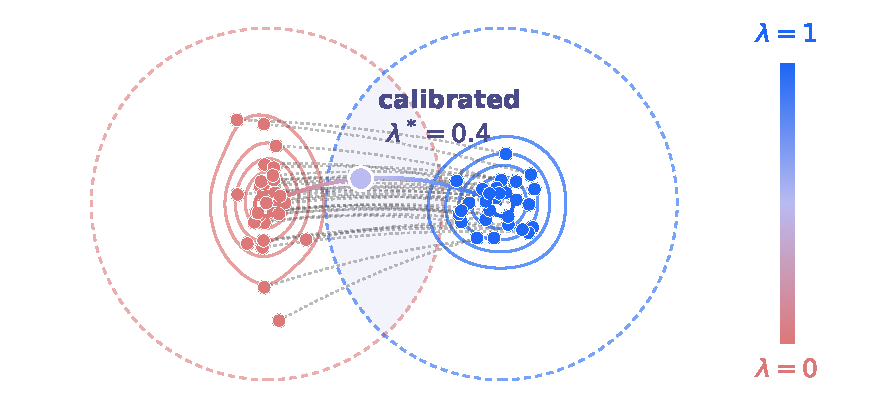
\includegraphics[trim={1.5cm 0.4cm 0.9cm 0.4cm},clip,width=0.45\linewidth]{Figures/conceptual_sketch_tradeoff_compact.pdf}
    \caption{\textbf{Certified lens and optimal-transport coupling.} The dashed ellipses show the certified lens $\mathcal{C}$, centered at base CF-distribution $\mathbb{P}_{\mathrm{CF}}$ (pink) and observed target-class distribution $\mathbb{P}_1$ (teal) with radii $\delta$ and $\epsilon$. The shaded intersection is $\mathcal{C}$. Dashed lines show the optimal coupling $\pi^\star$ between the two empirical distributions, and the purple marker shows the calibrated barycenter $\mathbb{Q}(\lambda^\star)$ realized along this coupling, positioned inside the lens.}
    \label{fig:conceptual}
\end{figure}

\begin{proof}[Proof sketch]
For any $\mu\in\mathcal{C}$, the lens constraints and triangle
inequality give
$
W_2(\mathbb{Q},\mu)
\le
\min\!\left\{
W_2(\mathbb{Q},\mathbb{P}_{\mathrm{CF}})+\delta,\,
W_2(\mathbb{Q},\mathbb{P}_1)+\epsilon
\right\}.
$
A convex relaxation followed by Young's inequality yields a family
of valid upper bounds whose $\mathbb{Q}$-dependent terms are positive
weighted sums of
$W_2^2(\mathbb{Q},\mathbb{P}_{\mathrm{CF}})$ and
$W_2^2(\mathbb{Q},\mathbb{P}_1)$.
After normalization, their minimizers take the barycentric form in
Eq.~\ref{eq:barycentric_family}.
The admissible bounds span $\lambda\in[0,1]$.
See Appendix~\ref{app:barycentric_bound} for the full proof.
\end{proof}

%Proposition~\ref{prop:barycentric_family} certifies a family of candidates, not a single optimum: 
Each $\mathbb{Q}(\lambda)$ minimizes a valid upper bound on $R(\mathbb{Q})$, not necessarily $R(\mathbb{Q})$ itself. %, nor that the bound is tight. 
%Proposition~\ref{prop:barycentric_family} does not assert that every
%$\mathbb{Q}(\lambda)$ directly minimizes the original worst-case risk
%$R(\mathbb{Q})$. Rather, it shows that the lens induces a family of
%\emph{certified barycentric candidates}, each minimizing a valid
%upper bound on $R(\mathbb{Q})$. 
The remaining question is therefore not where to search for a robust refinement, but where to locate the refinement along this certified path, which we answer by evaluating $\Phi_r$ directly, rather than continuing to rely on the bound.

\begin{corollary}[Geodesic characterization]
\label{cor:geodesic_characterization}
Let $D=W_2(\mathbb{P}_{\mathrm{CF}},\mathbb{P}_1)$.
At the endpoints, $\mathbb{Q}(0)= \mathbb{P}_\mathrm{CF}$ and $\mathbb{Q}(1)= \mathbb{P}_\mathrm{1}$ trivially.
For any $\lambda\in(0,1)$, every minimizer of Eq.~\ref{eq:barycentric_family2} lies at time $\lambda$ on a constant-speed $W_2$ geodesic between $\mathbb{P}_{\mathrm{CF}}$ and $\mathbb{P}_1$. In particular,
\begin{equation}
W_2(\mathbb{Q}(\lambda),\mathbb{P}_{\mathrm{CF}})
=
\lambda D,
\qquad
W_2(\mathbb{Q}(\lambda),\mathbb{P}_1)
=
(1-\lambda)D.
\label{eq:geodesic_distances}
\end{equation}
%Conversely, every time-$\lambda$ point on such a geodesic minimizes Eq.~\ref{eq:barycentric_family}.
If the optimal coupling between $\mathbb{P}_{\mathrm{CF}}$ and $\mathbb{P}_1$ is unique, then $\mathbb{Q}(\lambda)$ is unique for every $\lambda\in(0,1)$, and the barycentric parameter $\lambda$ coincides with the \textcolor{frappe_red}{consistency}--plausibility parameter of Proposition~\ref{prop:cf-tradeoff}.
\end{corollary}

Combining Corollary~\ref{cor:geodesic_characterization} with Proposition~\ref{prop:cf-tradeoff} gives
$
\mathbb{Q}(\lambda)\in\mathcal{C}
\Longleftrightarrow
\lambda D\leq\delta
\;\text{ and }\;
(1-\lambda)D\leq\epsilon.
$
%Using this geometry, we obtain a structural bound on how far any calibrated $\mathbb Q(\lambda^\star)$ can be from the unrestricted minimax risk $R^\star$, holding for \emph{every} admissible $(\epsilon,\delta)$, not a value we compute for a specific pair, without claiming $\lambda^\star$ is minimax-optimal. 

\color{black}
% \begin{corollary}[Geodesic characterization and conditional uniqueness]
% \label{cor:geodesic_characterization}
% Let $D=W_2(\mathbb{P}_{\mathrm{CF}},\mathbb{P}_1)$.
% At the endpoints, $\mathbb{Q}(0)= \mathbb{P}_\mathrm{CF}$ and $\mathbb{Q}(1)= \mathbb{P}_\mathrm{1}$ trivially.
% For any $\lambda\in(0,1)$, every minimizer of Eq.~\ref{eq:barycentric_family} lies at time $\lambda$ on a constant-speed $W_2$ geodesic between $\mathbb{P}_{\mathrm{CF}}$ and $\mathbb{P}_1$. In particular,
% \begin{equation}
% W_2(\mathbb{Q}(\lambda),\mathbb{P}_{\mathrm{CF}})
% =
% \lambda D,
% \qquad
% W_2(\mathbb{Q}(\lambda),\mathbb{P}_1)
% =
% (1-\lambda)D.
% \label{eq:geodesic_distances}
% \end{equation}
% Conversely, every time-$\lambda$ point on such a geodesic minimizes Eq.~\ref{eq:barycentric_family}.
% If the optimal coupling between $\mathbb{P}_{\mathrm{CF}}$ and $\mathbb{P}_1$ is unique, then $\mathbb{Q}(\lambda)$ is unique for every $\lambda\in(0,1)$, and the bound family induces a unique displacement path between the two anchors. 
% Thus, the barycentric parameter $\lambda$ coincides with the proximity--plausibility parameter of Proposition~\ref{prop:cf-tradeoff}.
% \end{corollary}

% Combining Corollary~\ref{cor:geodesic_characterization} with Proposition~\ref{prop:cf-tradeoff} gives
% \begin{equation}
% \mathbb{Q}(\lambda)\in\mathcal{C}
% \quad\Longleftrightarrow\quad
% \lambda D\leq\delta
% \;\text{ and }\;
% (1-\lambda)D\leq\epsilon,
% \label{eq:barycentric_lens_membership}
% \end{equation}
% or equivalently,
% $\lambda
% \in
% \left[
% 1-\frac{\epsilon}{D},
% \frac{\delta}{D}
% \right]\cap[0,1]$.



\textbf{Geometry versus certificate.}
The two anchors $\mathbb{P}_{\mathrm{CF}}$ and $\mathbb{P}_1$ determine the \emph{direction} of the barycentric refinement: $\lambda=0$ recovers the original CF distribution, $\lambda=1$ gives full alignment with target class distribution, and intermediate values trade off generator-specific CF geometry against target-side alignment.
The lens radii $\epsilon$ and $\delta$ instead provide the theoretical certificate: they determine the admissible \textcolor{frappe_red}{consistency}--plausibility range and the resulting robust-risk guarantees, without affecting which geodesic the refinement moves along or requiring any numerical instantiation. 
The decoupling matters in operation: it means that the search direction is fixed by the generator and the data as soon as $G$ and $\mathbb{P}_1$ are given, while the choice of \emph{where} along that direction to certify is a separate, data-driven calibration problem.
%Certification of the entire path does not imply every $\lambda$ is equally desirable; it identifies a theoretically justified search family, not an operating point, since the two anchors alone cannot determine the future distribution that $\mathbb{P}_1$ only approximates.
%We thus use held-out proxy deployment shifts to select $\lambda^\star$ along the certified path.

%In particular, Proposition~\ref{prop:cf-tradeoff} characterizes how $\epsilon$ and $\delta$ constrain the Wasserstein path between $\mathbb{P}_{\mathrm{CF}}$ and $\mathbb{P}_1$, whereas Proposition~\ref{prop:barycentric_family} shows that the robust relaxation induces candidates along this two-anchor path. Thus, the radii determine the admissible uncertainty and certificate, while the anchors determine the candidate refinement geometry.
%The lens radii $\epsilon$ and $\delta$ affect the value and tightness of the resulting robust upper bounds, but not their $\mathbb{Q}$-dependent minimization geometry. In particular, the radii enter the additive certificate terms in the bound, whereas the two anchors determine the barycentric geodesic characterized above. Thus, Proposition~\ref{prop:barycentric_family} should not be interpreted as claiming that $\mathbb{Q}(\lambda)$ solves the original minimax problem in Eq.~\ref{eq:intractable_objective}. Rather, the robust analysis reduces the unrestricted search over $\mathcal{P}_2(\mathcal X)$ to a one-dimensional, two-anchor barycentric candidate geometry.

%The endpoints have a direct interpretation:
%$\lambda=0$ recovers the original CF distribution
%$\mathbb{P}_{\mathrm{CF}}$, whereas $\lambda=1$ corresponds to full
%alignment with the observed target distribution $\mathbb{P}_1$.
%Intermediate values trade off preservation of the generator-specific
%counterfactual geometry against target-side alignment. 
%Certification of the entire path does not imply that all values of $\lambda$ are equally desirable; it identifies a theoretically justified search
%family, while the appropriate operating point depends on deployment
%evidence. The two anchors alone cannot determine this operating point:
%$\mathbb{P}_{\mathrm{CF}}$ reflects the current generator, whereas
%$\mathbb{P}_1$ reflects the observed target population rather than
%the unknown future one. We therefore use held-out proxy deployment
%shifts in Section~\ref{sec:calibration} to select
%$\lambda^\star$ along the certified path.

% \subsection{Deployment Calibration along the Certified Path}
% \label{sec:calibration}

% We use a held-out calibration set containing $M$ proxy deployment
% environments. Let $\widehat{\mu}_m$, $m=1,\ldots,M$, denote the
% target-side reference distribution under the $m$-th proxy shift.
% These calibration distributions are used only for calibration and
% are disjoint from the shifted environments used for final evaluation.

%\textbf{Lens calibration.}
%For a user-specified miscoverage level $\alpha_{\mathrm{cal}}\in(0,1)$, we calibrate the two lens radii using empirical distance quantiles:
%\begin{equation}\label{eq:radii_calibration}
%\delta
%=
%\operatorname{Quantile}_{1-\alpha_{\mathrm{cal}}}
%\left(
%\left\{
%W_2(\widehat{\mu}_m,\mathbb{P}_{\mathrm{CF}})
%\right\}_{m=1}^M
%\right),
% \quad
% \epsilon
% =
% \operatorname{Quantile}_{1-\alpha_{\mathrm{cal}}}
% \left(
% \left\{
% W_2(\widehat{\mu}_m,\mathbb{P}_1)
% \right\}_{m=1}^M
% \right).
% \end{equation}
% By construction, each radius individually covers a ($1-\alpha_{\mathrm{cal}}$) fraction of the proxy deployment distributions with respect to its own anchor. By a union bound, the lens $\mathcal{C}$ jointly covers at least a $(1-2\alpha_{\mathrm{cal}})$ fraction.
% %Thus, the lens is calibrated to cover a prescribed fraction of the
% %proxy deployment distributions. 
% We additionally enforce
% $
% \epsilon+\delta
% \ge
% W_2(\mathbb{P}_{\mathrm{CF}},\mathbb{P}_1)
% $
% to ensure that the lens is nonempty.

% \textbf{Path calibration.}
% Proposition~\ref{prop:barycentric_family} reduces the refinement
% search to the certified barycentric family
% $\{\mathbb{Q}(\lambda):\lambda\in[0,1]\}$.
% We select the member that minimizes the worst-case mismatch over the
% held-out proxy shifts:
% \begin{equation}
% \widehat{R}_{\mathrm{cal}}(\lambda)
% :=
% \max_{m=1,\ldots,M}
% W_2^2\!\left(
% \mathbb{Q}(\lambda),\widehat{\mu}_m
% \right),
% \label{eq:proxy_risk}
% \end{equation}
% \begin{equation}
% \lambda^\star
% \in
% \arg\min_{\lambda\in[0,1]}
% \widehat{R}_{\mathrm{cal}}(\lambda).
% \label{eq:lambda_calibration}
% \end{equation}
% The resulting $\mathbb{Q}(\lambda^\star)$ is therefore the member of the certified barycentric family that is most robust to the observed proxy deployment shifts. 
% Importantly, the proxy shifts used for this selection are held out from the final evaluation environments.

\iffalse
\subsection{Deployment-Stress Calibration}
\label{sec:calibration}

Section~\ref{sec:barycentric} reduces the unrestricted refinement problem to the one-dimensional barycentric family $\{\mathbb{Q}(\lambda):\lambda\in[0,1]\}$, whose parameter $\lambda$ has the exact \textcolor{frappe_red}{consistency}--plausibility interpretation established in Proposition~\ref{prop:cf-tradeoff}.
The robust analysis therefore determines a theoretically justified candidate geometry, but does not prescribe which operating point along this path should be deployed.
Since the realized deployment shift is unknown at construction time, we select the operating point using held-out calibration factuals evaluated under radius-specific adversarial model updates constructed from the training split.

% \textbf{Calibration stresses.}
% We construct $M$ stressed calibration datasets 
% $\mathcal{D}_{\mathrm{cal}}^{(m)}=\left\{\xi_i+\Delta_i^{(m)}\right\}_{i=1}^{N}$,
% $m=1,\ldots,M$ from a held-out split $\mathcal{D}_{\mathrm{cal}}=\{\xi_i\}_{i=1}^{N}$,
% where each perturbation satisfies a common transport budget $\frac{1}{N}\sum_{i=1}^{N}\left\|\Delta_i^{(m)}\right\|_2^2 \le b_{\mathrm{cal}}^2$.
% We set $b_{\mathrm{cal}}$ via a standard bootstrap procedure: letting $\widehat{\mathbb{P}}_{\mathrm{cal}}=\frac{1}{N}\sum_{i=1}^{N}\delta_{\xi_i}$ be the empirical calibration distribution and $\widehat{\mathbb{P}}_{\mathrm{cal}}^{*(r)}$,$r=1,\dots,B$ its bootstrap resamples,
% \begin{equation}
% b_{\mathrm{cal}}
% =
% \operatorname{Quantile}_{1-\alpha}
% \left\{
% W_2\!\left(
% \widehat{\mathbb{P}}_{\mathrm{cal}}^{*(r)},
% \widehat{\mathbb{P}}_{\mathrm{cal}}
% \right)
% \right\}_{r=1}^{B}.
% \label{eq:bootstrap_budget}
% \end{equation}
% This gives an evaluation-free reference scale for local stresses; it is not an estimate of the realized future distribution shift.


\textbf{Held-out calibration.}
We use a held-out split
$\mathcal{D}_{\mathrm{cal}}=\{\xi_i\}_{i=1}^{N}$
only to select refinement operating points for robustness configurations
constructed from the training split. In particular, the calibration data are
not used to construct an additional ambiguity set, generate new
distributional stresses, or update the corresponding adverse models.
All adverse model-update configurations and refinement geometries are frozen
before the calibration split is accessed. We first restrict calibration to factual instances that are unfavorable under
the current classifier,
$
\mathcal{I}_{\mathrm{cal}}
:=
\left\{
i:
f_0(x_i^{\mathrm{cal}})<\tau
\right\}.
$
For each $i\in\mathcal{I}_{\mathrm{cal}}$, the unchanged base generator
produces
$
z_i^{\mathrm{cal}}
=
G(x_i^{\mathrm{cal}}).
$
Only successful CFs satisfying
$f_0(z_i^{\mathrm{cal}})\geq\tau$
are retained. For a candidate refinement depth $\lambda$, each retained
base CF is refined using the same frozen rule as in training,
$
z_i^{\mathrm{cal}}(\lambda)
=
\operatorname{Refine}_{\lambda}
\bigl(z_i^{\mathrm{cal}}\bigr).
$
No model is updated at this stage; the refined calibration CFs are evaluated
under adverse model-update configurations constructed exclusively from the
training split.

\textbf{Within-radius operating-point calibration.}
For each uncertainty radius $r\in\mathcal{R}$, let
$\mathcal{F}_{r}^{\mathrm{adv}}$
denote the corresponding frozen family of adverse fine-tuned models. We define
the held-out calibration invalidity at refinement depth $\lambda$ as
\begin{equation}
\widehat L_{\mathrm{cal}}(r,\lambda)
:=
\max_{f\in\mathcal{F}_{r}^{\mathrm{adv}}}
\frac{1}{|\mathcal{I}_{\mathrm{cal}}^{\mathrm{valid}}|}
\sum_{i\in\mathcal{I}_{\mathrm{cal}}^{\mathrm{valid}}}
\left[
\tau
-
f\!\left(
z_i^{\mathrm{cal}}(\lambda)
\right)
\right]_+ ,
\label{eq:heldout_calibration_invalidity}
\end{equation}
where
$\mathcal{I}_{\mathrm{cal}}^{\mathrm{valid}}$
contains the calibration factuals for which the base generator returns a
current-valid CF. Together with the corresponding recourse cost
$C_{\mathrm{cal}}(\lambda)$, this defines, for each fixed $r$, a
robustness--\textcolor{frappe_red}{consistency} trade-off over $\lambda$. A predefined frontier
operating-point rule selects
\[
\lambda_r^\star
\in
\operatorname{SelectFrontier}
\left\{
\bigl(
C_{\mathrm{cal}}(\lambda),
\widehat L_{\mathrm{cal}}(r,\lambda)
\bigr)
:
\lambda\in\Lambda
\right\},
\]
where lower recourse cost and lower calibration invalidity are preferred.

\textbf{Cross-radius validation.}
The resulting configurations
$\{(r,\lambda_r^\star):r\in\mathcal{R}\}$
are subsequently evaluated on a disjoint shift-validation set whose
realizations are not used in the within-radius selection of
$\lambda_r^\star$. This second stage compares uncertainty coverage against
held-out robustness across radii and selects the final radius
$r^\star$ using a predefined coverage--validity trade-off rule. The deployed
refinement depth is then fixed as
$\lambda_{r^\star}^\star$.
No information from the final future-shift test set is used in either the
within-radius calibration of $\lambda$ or the cross-radius selection of $r$.
%Let
%$\mathcal{D}_{\mathrm{cal}}=\{\xi_i\}_{i=1}^{N}$
%denote a held-out calibration split that is not used for evaluation.
%We construct $M$ stressed calibration datasets
%\begin{equation}
%\mathcal{D}_{\mathrm{cal}}^{(m)}
%=
%\left\{
%\xi_i+\Delta_i^{(m)}
%\right\}_{i=1}^{N},
%\qquad
%m=1,\ldots,M,
%\label{eq:calibration_stresses}
%\end{equation}
%where each perturbation satisfies the common transport budget
%\begin{equation}
%\frac{1}{N}
%\sum_{i=1}^{N}
%\left\|
%\Delta_i^{(m)}
%\right\|_2^2
%\le
%b_{\mathrm{cal}}^2.
%\label{eq:calibration_budget}
%\end{equation}
%Here, $b_{\mathrm{cal}}$ is a data-dependent local stress scale, not an estimate of the magnitude or direction of the realized future deployment shift.

%\textbf{Data-driven stress scale.}
%We determine $b_{\mathrm{cal}}$ exclusively from $\mathcal{D}_{\mathrm{cal}}$, without access to any evaluation shift.
%Let
%\[
%\widehat{\mathbb{P}}_{\mathrm{cal}}
%=
%\frac{1}{N}
%\sum_{i=1}^{N}
%\delta_{\xi_i}
%\]
%denote the empirical calibration distribution, and let
%$\widehat{\mathbb{P}}_{\mathrm{cal}}^{*(r)}$,
%$r=1,\ldots,B$, denote empirical distributions obtained from
%bootstrap resamples of $\mathcal{D}_{\mathrm{cal}}$.
%We set
% \begin{equation}
% b_{\mathrm{cal}}
% =
% \operatorname{Quantile}_{1-\alpha}
% \left\{
% W_2\!\left(
% \widehat{\mathbb{P}}_{\mathrm{cal}}^{*(r)},
% \widehat{\mathbb{P}}_{\mathrm{cal}}
% \right)
% \right\}_{r=1}^{B}.
% \label{eq:bootstrap_budget}
% \end{equation}
%Thus, bootstrap variability is used only to establish an evaluation-free reference scale for local stresses; it is not used to predict the realized future distribution shift or to select $\lambda$ directly.

% \textbf{Proxy deployment models.}
% Within this budget, we generate stress directions $\Delta^{(1)},\ldots,\Delta^{(M)}$ and retrain the predictive model on each stressed datasets using the original training procedure, 
% %This yields
% $
% f^{(m)}
% =
% \operatorname{Train}
% \left(
% \mathcal{D}_{\mathrm{train}}
% \cup
% \mathcal{D}_{\mathrm{cal}}^{(m)}
% \right)$,
% %\qquad
% $m=1,\ldots,M$,
% %\label{eq:proxy_models}
% %\end{equation}
% with the stress-generation procedure detailed in Section~\textcolor{latte_maroon}{add label}\ref{sec:experimental_setup}.
% %where the precise stress-generation procedure is given in Section~\ref{sec:experimental_setup}.
% The resulting models $f^{(1)},\ldots,f^{(M)}$ are not predictions of the realized future classifier, but proxies that probe the sensitivity to controlled local model updates.
% %Rather, they serve as proxy deployment models that probe the
% %sensitivity of candidate refinements to controlled local model
% %updates.

% \textbf{Operating-point selection.}
% For each candidate $\lambda$, we evaluate the corresponding barycentric distribution $\mathbb{Q}(\lambda)$ under all $M$ proxy models. %deployment shifts. 
% Using the margin-based invalidity surrogate $\ell_f(z)
% =
% [\tau-f(z)]_+$, 
% %\begin{equation}
% %\ell_f(z)
% %=
% %[\tau-f(z)]_+,
% %\label{eq:calibration_loss}
% %\end{equation}
% we define the worst-case calibration risk
% \begin{equation}
% \widehat{R}_{\mathrm{cal}}(\lambda)
% =
% \max_{m\in[M]}
% \mathbb{E}_{z\sim\mathbb{Q}(\lambda)}
% \left[
% \ell_{f^{(m)}}(z)
% \right].
% \label{eq:calibration_risk}
% \end{equation}
% Lower values of $\widehat{R}_{\mathrm{cal}}(\lambda)$ indicate greater robustness to the deployment shifts.


\iffalse
Importantly, we do not select $\lambda$ by minimizing $\widehat{R}_{\mathrm{cal}}(\lambda)$ alone:
this can favor large values of $\lambda$, since moving toward the target anchor may keep improving robustness while incurring increasingly large departures from the \textcolor{frappe_red}{consistent} anchor. 
Instead, using the geodesic characterization in $W_2\!\left(
\mathbb{Q}(\lambda),
\mathbb{P}_{\mathrm{CF}}
\right)
=
\lambda D$ (with $D
:=
W_2(\mathbb{P}_{\mathrm{CF}},\mathbb{P}_1)$), 
so $\lambda$ itself is the normalized refinement depth, we select an operating point on the
robustness--refinement frontier.

%Section~\ref{sec:barycentric} to make this additional refinement
%explicit. Since
%$
%D
%:=
%W_2(\mathbb{P}_{\mathrm{CF}},\mathbb{P}_1),
%$
%along the barycentric path,
%$
%W_2\!\left(
%\mathbb{Q}(\lambda),
%\mathbb{P}_{\mathrm{CF}}
%\right)
%=
%\lambda D,
%\label{eq:refinement_cost}
%$
%$\lambda$ itself is the normalized refinement depth from the proximal anchor.
%We therefore select an operating point on the
%robustness--refinement frontier rather than the point of maximal robustness. %Specifically, relative to the unrefined counterfactual
We define the normalized robustness gain relative to the unrefined CF population,
% population, define the normalized robustness gain
\begin{equation}
 G_{\mathrm{cal}}(\lambda)
 =
 \frac{
 \widehat{R}_{\mathrm{cal}}(0)
 -
 \widehat{R}_{\mathrm{cal}}(\lambda)
 }{
 \widehat{R}_{\mathrm{cal}}(0)+\xi
 },
 \label{eq:calibration_gain}
 \end{equation}
 with small constant $\xi>0$, and choose
% where $\xi>0$ is a small numerical constant. We choose
 \begin{equation}
 \lambda^\star
 \in
 \arg\max_{\lambda\in\Lambda}
 \left\{
 G_{\mathrm{cal}}(\lambda)-\lambda
 \right\},
 \label{eq:lambda_calibration}
 \end{equation}
 over a fixed grid $\Lambda\subset[0,1]$, ties are resolved towards the smallest $\lambda$.
% where $\Lambda\subset[0,1]$ is a fixed one-dimensional grid.
% Ties are resolved in favor of the smallest $\lambda$.
This is a parsimonious stopping rule:
% Equation~\ref{eq:lambda_calibration} implements a parsimonious
% stopping rule: 
refinement is favored only when its robustness gain is commensurate with the additional displacement from the \textcolor{frappe_red}{consistent} anchor.
% the proximal anchor. 
Consequently, $\lambda^\star$ does not intended to maximize robustness irrespective of cost, nor is $\lambda=1$ privileged, it identifies the point at which no further movement toward the target anchor yields insufficient calibration benefit relative to the refinement required. 
%an efficient
% operating point at which further movement toward the target anchor
% provides insufficient calibration benefit relative to the
% additional refinement it requires.

% This separates the roles of theory and deployment calibration.
% The robust analysis in Section~\ref{sec:barycentric} determines
% the candidate geometry and gives $\lambda$ an exact interpretation
% as normalized refinement depth, whereas held-out deployment
% stresses determine how much of that refinement is warranted.
The only refinement parameter selected for deployment is the scalar $\lambda^\star$.
\fi
\begin{proposition}[A posteriori robust-risk certificate]
\label{prop:suboptimality}
Suppose the lens $\mathcal C$ is nonempty, i.e.,
$\delta+\epsilon\ge D$.
Define
$
L_{\mathcal C}
=
\min(D,\delta)+\min(D,\epsilon)-D,
$
and let
$
R^\star
=
\inf_{\mathbb Q\in\mathbb P_2(\mathcal X)}
\sup_{\mu\in\mathcal C}
W_2^2(\mathbb Q,\mu).
$
Then
$
R^\star
\ge
\frac{L_{\mathcal C}^2}{4}.
$
Moreover, for every $\mathbb Q(\lambda)$ in the barycentric
family,
\[
R(\mathbb Q(\lambda))
\le
\min\left\{
(\lambda D+\delta)^2,\,
((1-\lambda)D+\epsilon)^2
\right\}.
\]
so for any calibrated operating point $\lambda^\star$,
\[
0
\le
R(\mathbb Q(\lambda^\star))-R^\star
\le
\min\left\{
(\lambda^\star D+\delta)^2,\,
((1-\lambda^\star)D+\epsilon)^2
\right\}
-
\frac{L_{\mathcal C}^2}{4}.
\]
\end{proposition}

The lower bound follows since a nonempty lens contains a segment of length $L_{\mathcal C}=\min(D,\delta)+\min(D,\epsilon)-D$ of the geodesic connecting the \textcolor{frappe_red}{consistent} anchor
$\mathbb{P}_{\mathrm{CF}}$ and the plausible anchor $\mathbb{P}_1$, so any center must lie at least $L_{\mathcal C}/2$ away from one endpoints of this segment. The upper bound for $\mathbb Q(\lambda)$ follows from the geodesic identities and the triangle inequality. 
Proposition~\ref{prop:suboptimality} does not require the calibrated operating point $\lambda^\star$ to minimize the original minimax objective, calibration trades off robustness against refinement cost, while Eq.~\ref{eq:intractable_objective} ignores that cost entirely.
It instead gives an explicit, computable upper
bound
$R(\mathbb Q(\lambda))
\le
\min\{(\lambda D+\delta)^2,
((1-\lambda)D+\epsilon)^2\}$, on how far the calibrated solution's worst-case risk can be from the unrestricted minimax optimum, without claiming that $\lambda^\star$ is minimax-optimal or that the upper bound is tight.
\fi

\subsection{Data-Side Wasserstein Robust Operating-Point Selection}\label{subsec:wro}
We select the deployed $\lambda$ by evaluating $\Phi_r$ directly on the reduced family $\{\mathbb Q(\lambda):\lambda\in[0,1]\}$, writing $\Phi_r(\lambda) := \Phi_r(\mathbb Q(\lambda))$, rather than continuing to rely on the proxy $R$.
Consequently, we do not need a separate $R$-based suboptimality certificate here: Proposition~\ref{prob:future-validity} already certifies that reducing $R$ tightens the bound on $\Phi_r$, and Section~\ref{sec:stability} bounds the grid-search error directly against $\Phi_r$, the quantity actually optimized.
%Recall from Section~\ref{sec:objective} the data-side uncertainty set $\mathcal U_r$ and the update-induced score $f_\mathbb{P}=\operatorname{Update}(f_0,\mathbb{P})$ for $\mathbb{P}\in\mathcal U_r$. 
For a fixed radius $r$ and refinement depth$\lambda$, the robust operating point is
\[
\lambda_r^\star \in \arg\min_{\lambda\in[0,1]} \Phi_r(\lambda),
\qquad
\Phi_r(\lambda) = \sup_{\mathbb{P}\in\mathcal U_r} \mathbb E_{z\sim\mathbb{Q}(\lambda)}\left[\ell_{f_\mathbb{P}}(z)\right].
\]
% We now select the operating point on this path according to robustness
% against future model updates induced by distribution shift.
% For a Wasserstein uncertainty radius $r\ge 0$, define the data-side
% uncertainty set
% $
% \mathcal U_r
% =
% \left\{
% P:
% W_{\mathrm{data}}(P,\widehat P_{\mathrm{tr}})\le r
% \right\}.
% $
% For each shifted training distribution $P\in\mathcal U_r$, let
% $
% f_P
% =
% \operatorname{Update}(f_0,P)
% $
% denote the classifier obtained by applying the fixed model-update
% procedure to the current classifier $f_0$. In our primary implementation,
% $\operatorname{Update}$ corresponds to fine-tuning from $f_0$.
% Let
% $
% \ell_f(z)
% =
% [\tau-f(z)]_+
% $
% denote the margin-based counterfactual invalidity loss. For a fixed
% uncertainty radius $r$ and refinement depth $\lambda$, we define the
% worst-case future counterfactual risk
% $
% \Phi_r(\lambda)
% :=
% \sup_{P\in\mathcal U_r}
% \mathbb E_{z\sim Q(\lambda)}
% \left[
% \ell_{f_P}(z)
% \right].
% $
% Thus, $r$ specifies the admissible magnitude of future data shift,
% whereas $\lambda$ is the decision variable controlling the refinement
% depth along the barycentric path.
% The robust operating point for radius $r$ is therefore
% $
% \lambda_r^\star
% \in
% \arg\min_{\lambda\in[0,1]}
% \Phi_r(\lambda).
% $

\paragraph{Approximate inner maximization.}
The supremum defining $\Phi_r(\lambda)$ is generally intractable because
each candidate distribution $\mathbb{P}$ induces a model update before its
counterfactual loss can be evaluated. We therefore approximate the inner
problem by constructing, for every pair $(r,\lambda)$, an adversarial
training distribution
$
\mathbb{P}_{r,\lambda}^{\mathrm{adv}}
\approx
\arg\max_{\mathbb{P}\in\mathcal U_r}
\mathbb E_{z\sim Q(\lambda)}
\left[
\ell_{\operatorname{Update}(f_0,\mathbb{P})}(z)
\right].
$
%The corresponding adverse future model is
$
f_{r,\lambda}^{\mathrm{adv}}
=
\operatorname{Update}
\left(
f_0,
\mathbb{P}_{r,\lambda}^{\mathrm{adv}}
\right).
$
Importantly, the adversarial distribution is conditioned on both the
uncertainty radius and the refinement depth. Different members $Q(\lambda)$ of the barycentric family may therefore induce different worst-case future shifts.

\paragraph{Held-out estimation and cross-radius selection.}
On a held-out calibration split $\mathcal D_{\mathrm{cal}}$, not used to construct the adversarial training distributions, we estimate  %For each candidate $\lambda$, we refine the current-valid base counterfactuals using the frozen refinement rule and estimate
$
\widehat\Phi_r(\lambda)
=
\frac{1}{|I_{\mathrm{cal}}^{\mathrm{valid}}|}
\sum_{i\in I_{\mathrm{cal}}^{\mathrm{valid}}}
\left[
\tau-
f_{r,\lambda}^{\mathrm{adv}}
\left(
z_i^{\mathrm{cal}}(\lambda)
\right)
\right]_+ 
$ over a grid $\Lambda\subset[0,1]$ and take $
\widehat\lambda_r
\in
\arg\min_{\lambda\in\Lambda}
\widehat\Phi_r(\lambda),
$
as the empirical robust operating point. 
% is then selected as
%$
%\widehat\lambda_r
%\in
%\arg\min_{\lambda\in\Lambda}
%\widehat\Phi_r(\lambda),
%$
%where $\Lambda\subset[0,1]$ is the predefined one-dimensional search grid.
%\paragraph{Cross-radius selection.}
The resulting configurations
$
\{(r,\widehat\lambda_r):r\in\mathcal R\}
$
are subsequently evaluated on a disjoint shift-validation split to
select the final uncertainty radius $r^\star$. The deployed refinement
depth is then fixed as
$
\lambda^\star
=
\widehat\lambda_{r^\star}.
$


% . This distinction is deliberate: calibration selects
% $\lambda^\star$ according to the robustness--refinement trade-off,
% whereas Eq.~\ref{eq:intractable_objective} minimizes worst-case
% distributional risk irrespective of the amount of additional
% refinement. The proposition instead provides an \emph{a posteriori} certificate
% for the selected operating point. Since the lens is
% nonempty, it necessarily contains a segment of the Wasserstein
% geodesic connecting the proximal anchor
% $\mathbb{P}_{\mathrm{CF}}$ and the target anchor $\mathbb{P}_1$.
% The length of this contained segment is
% $L_{\mathcal C}=\min(D,\delta)+\min(D,\epsilon)-D$.
% Any distribution $\mathbb Q$ serving as a center of the lens must
% therefore be at least $L_{\mathcal C}/2$ away from one of the two
% endpoints of this segment. Consequently, the unrestricted minimax
% risk $R^\star$ satisfies
% $R^\star\ge L_{\mathcal C}^2/4$.

% For a barycentric candidate $\mathbb Q(\lambda)$, the exact geodesic
% identities
% $W_2(\mathbb Q(\lambda),\mathbb P_{\mathrm{CF}})=\lambda D$
% and
% $W_2(\mathbb Q(\lambda),\mathbb P_1)=(1-\lambda)D$,
% together with the triangle inequality, give the computable upper
% bound
% $R(\mathbb Q(\lambda))
% \le
% \min\{(\lambda D+\delta)^2,
% ((1-\lambda)D+\epsilon)^2\}$.
% Evaluating this bound at the calibrated operating point
% $\lambda^\star$ and combining it with the lower bound on $R^\star$
% yields
% $0\le
% R(\mathbb Q(\lambda^\star))-R^\star
% \le
% \min\{(\lambda^\star D+\delta)^2,
% ((1-\lambda^\star)D+\epsilon)^2\}
% -L_{\mathcal C}^2/4$.

% Thus, calibration and certification play complementary roles.
% Calibration determines how far refinement is worth pursuing, while
% Proposition~\ref{prop:suboptimality} certifies the resulting choice
% after the operating point has been selected. In particular, the
% result does not claim that $\lambda^\star$ is minimax-optimal or that
% the upper bound is tight. Rather, it provides an explicit upper bound
% on how far the worst-case lens risk of the calibrated solution can be
% from the unrestricted minimax optimum.
\subsection{Stability of the One-Dimensional Robust Objective}\label{sec:stability}
Section~\ref{subsec:wro} approximates $\lambda_r^\star=\arg\min_{\lambda\in[0,1]}\Phi_r(\lambda)$ by evaluating $\Phi_r$ on a finite grid $\Lambda\subset[0,1]$ rather than solving the continuous minimization exactly.
This only holds if $\Phi_r$ varies with $\lambda$ in a controlled manner; we thus now show that $\Phi_r$ is Lipschitz continuous in $\lambda$, and derive an explicit bound on the supoptimality introduced by the finite-grid search.
%We now show that the geometry induced by the barycentric family makes
%this robust objective $\Phi_r$ stable with respect to the one-dimensional
%refinement parameter $\lambda$.

%\paragraph{Uniform Lipschitz condition.}
%Assume that for a fixed uncertainty radius $r$, the future-model
%invalidity losses are uniformly Lipschitz over the data-side uncertainty
%set:
%$
%L_r
%:=
%\sup_{\mathbb{P}\in\mathcal U_r}
%\operatorname{Lip}(\ell_{f_\mathbb{P}})
%<
%\infty,
%$
%where the Lipschitz constant is measured with respect to the CF-side ground metric.

% Let
% $
% D
% =
% \textcolor{frappe_red}{W_{\mathrm{CF}}}(\mathbb{P}_{\mathrm{CF}},\mathbb{P}_1).
% $
% Since $\{Q(\lambda):\lambda\in[0,1]\}$ is a constant-speed
% Wasserstein geodesic between $\mathbb{P}_{\mathrm{CF}}$ and $\mathbb{P}_1$,
% $
% \textcolor{frappe_red}{W_{\mathrm{CF}}}
% \left(
% Q(\lambda),Q(\lambda')
% \right)
% =
% D|\lambda-\lambda'|\qquad\forall\,\lambda,\lambda'\in[0,1].
% $
\paragraph{Lipschitz continuity of $\Phi_r$ in $\lambda$.} Recall $L_r$ from Assumption~\ref{ass:update-lipschitz} (the uniform sensitivity of any reachable future score to displacement of its input) and $D=W_2(\mathbb P_{\mathrm{CF}},\mathbb P_1)$ from Proposition~\ref{prop:cf-tradeoff} (the length of the barycentric path).
\begin{proposition}[Lipschitz stability of the robust objective]
For any $\lambda,\lambda'\in[0,1]$,
\(
\left|
\Phi_r(\lambda)
-
\Phi_r(\lambda')
\right|
\le
L_r D
|\lambda-\lambda'|.
\)
Hence, $\Phi_r$ is Lipschitz continuous on $[0,1]$ and therefore admits
at least one robust operating point
$
\lambda_r^\star
\in
\arg\min_{\lambda\in[0,1]}
\Phi_r(\lambda).
$
\end{proposition}

\begin{proof}[Proof sketch]
Fix any $\mathbb{P}\in\mathcal U_r$. Lemma~\ref{lem:score-diff} bounds the resulting score difference between two points on the path: $|\mathbb E_{Q(\lambda)}[\ell_{f_\mathbb{P}}]-\mathbb E_{Q(\lambda')}[\ell_{f_\mathbb{P}}]|\le L_r\,W_2(Q(\lambda),Q(\lambda'))$. Because $\{Q(\lambda)\}$ is a constant-speed geodesic (Corollary~\ref{cor:geodesic_characterization}), $W_2(Q(\lambda),Q(\lambda'))=D|\lambda-\lambda'|$ exactly, so the bound becomes $L_rD|\lambda-\lambda'|$. This holds for every $\mathbb{P}\in\mathcal U_r$, so it also holds after taking the supremum over $\mathbb{P}$ that defines $\Phi_r$.
% For any fixed $\mathbb{P}\in\mathcal U_r$, the Kantorovich--Rubinstein
% inequality gives
% \[
% \left|
% \mathbb E_{Q(\lambda)}
% [\ell_{f_\mathbb{P}}]
% -
% \mathbb E_{Q(\lambda')}
% [\ell_{f_\mathbb{P}}]
% \right|
% \le
% L_r
% W_1
% \left(
% Q(\lambda),Q(\lambda')
% \right).
% \]
% Using $W_1\le \textcolor{frappe_red}{W_{\mathrm{CF}}}$ and the constant-speed geodesic identity,
% \[
% \left|
% \mathbb E_{Q(\lambda)}
% [\ell_{f_\mathbb{P}}]
% -
% \mathbb E_{Q(\lambda')}
% [\ell_{f_\mathbb{P}}]
% \right|
% \le
% L_rD|\lambda-\lambda'|.
% \]
% Taking the supremum over $\mathbb{P}\in\mathcal U_r$ on both sides yields the
% result.
\end{proof}
%\paragraph{Finite-grid optimization.}


\paragraph{Suboptimality of the finite-grid search.}
In practice, the operating point is selected over a finite grid
$
\Lambda_h
\subset[0,1],
$
of maximum spacing $h$, using
the approximate robust risk $
\widehat\Phi_r(\lambda)
$
obtained from the inner adversarial
solver. Assume that its uniform estimation
error over the search grid satisfies
$
\max_{\lambda\in\Lambda_h}
\left|
\widehat\Phi_r(\lambda)
-
\Phi_r(\lambda)
\right|
\le
\eta.
$
Let
$
\widehat\lambda_r
\in
\arg\min_{\lambda\in\Lambda_h}
\widehat\Phi_r(\lambda).
$
\begin{proposition}[Search error on the reduced decision path]
Under the assumptions above,
$
\Phi_r(\widehat\lambda_r)
\le
\min_{\lambda\in[0,1]}
\Phi_r(\lambda)
+
2\eta
+
\frac{L_rDh}{2}.
$
\end{proposition}

\begin{proof}[Proof sketch]
Let $\lambda_r^\star$ be a minimizer of $\Phi_r$ on $[0,1]$, and let
$\widetilde\lambda\in\Lambda_h$ be the closest grid point to
$\lambda_r^\star$. Then
$
|\widetilde\lambda-\lambda_r^\star|
\le
\frac h2.
$
By Lipschitz stability,
$
\Phi_r(\widetilde\lambda)
\le
\Phi_r(\lambda_r^\star)
+
\frac{L_rDh}{2}.
$
Using the uniform approximation error and the optimality of
$\widehat\lambda_r$ on the grid,
\[
\Phi_r(\widehat\lambda_r)
\le
\widehat\Phi_r(\widehat\lambda_r)+\eta
\le
\widehat\Phi_r(\widetilde\lambda)+\eta
\le
\Phi_r(\widetilde\lambda)+2\eta,
\]
which gives the stated bound.\end{proof}

\paragraph{Interpretation.}
The barycentric geometry derived in Section~3.2 does not itself define
deployment robustness; instead, it provides a one-dimensional decision
path on which the actual data-side Wasserstein robust risk is stable and
searchable. The bound above separates the two sources of numerical
suboptimality:
\[
\underbrace{2\eta}_{\text{inner-solver approximation}}
+
\underbrace{\frac{L_rDh}{2}}_{\text{one-dimensional discretization}}.
\]
Thus, finer search grids and stronger inner adversarial optimization
systematically tighten the quality of the selected operating point.





\subsection{OT Barycentric Realization}
\label{sec:transport}

Given the calibrated operating point $\lambda^\star$, we realize $Q(\lambda^\star)$ via optimal transport. 
Let $\{z_i\}_{i=1}^{n}$ and $\{y_j\}_{j=1}^{m}$ denote the empirical supports of
$\mathbb{P}_{\mathrm{CF}}$ and $\mathbb{P}_1$, and
$
\mathcal{F}_0
=
\{x : f_0(x) \ge \tau\}
$
the current favorable region. To keep transport path inside $\mathcal{F}_0$, we use the intrinsic distance
\[
d_{\mathcal{F}_0}(z,y)
=
\inf_{\substack{\gamma(0)=z,\ \gamma(1)=y\\
                 \gamma(t)\in\mathcal{F}_0,\ \forall t\in[0,1]}}
\int_0^1 \|\dot{\gamma}(t)\|_2\,dt.
\] and solve
\begin{equation}
\pi^\star
\in
\arg\min_{\pi\in\Pi(
\mathbb{P}_{\mathrm{CF}},\mathbb{P}_1)}
\sum_{i,j}
\pi_{ij}
d_{\mathcal{F}_0}^2(z_i,y_j),
\label{eq:optimal_transport}
\end{equation}
where
$\Pi(\mathbb{P}_{\mathrm{CF}},\mathbb{P}_1)$ denotes the set of
couplings with marginals
$\mathbb{P}_{\mathrm{CF}}$ and $\mathbb{P}_1$. %To ensure that the transport path from CFs toward the favorable population does not traverse regions classified as unfavorable by the current classifier, we measure transport intrinsically within the favorable region.
%In practice, $d_{\mathcal{F}_0}$ is approximated by shortest-path
%distances on a $k$-nearest-neighbor graph whose admissible edges remain
%within $\mathcal{F}_0$.
By construction $d_{\mathcal F_0}\ge\|\cdot\|_2$, with equality on $\mathcal F_0$ exactly when $\mathcal{F}_0$ is convex, i.e., 
%When $\mathcal{F}_0$ is convex, 
the straight-line segment between any
$z,y\in\mathcal{F}_0$ is feasible, in which case 
$d_{\mathcal{F}_0}(z,y)=\|z-y\|_2$.
%Hence, the proposed ground cost reduces exactly to the original quadratic Euclidean cost in this case. 
The refinement is the displacement
interpolation along the minimizing intrinsic transport paths:
%The refined counterfactual distribution is obtained by displacement interpolation along the minimizing intrinsic transport paths:
$
\mathbb{P}_{\mathrm{rCF}}
=
\sum_{i=1}^{n}
\sum_{j=1}^{m}
\pi_{ij}^\star
\,
\delta_{\gamma_{ij}^\star(\lambda^\star)},
\label{eq:refined_cf}
$
where $\gamma_{ij}^\star:[0,1]\rightarrow F_0$ is a constant-speed
$d_{F_0}$-minimizing geodesic from $z_i$ to $y_j$.
When $F_0$ is convex, $\gamma_{ij}^\star(\lambda)
=(1-\lambda)z_i+\lambda y_j$, recovering standard Euclidean
displacement interpolation.
By the equivalence between McCann displacement interpolation and the
two-measure Wasserstein barycenter
\citep{agueh2011barycenters},
$
\mathbb{P}_{\mathrm{rCF}}
=
\mathbb{Q}(\lambda^\star),
%\label{eq:realized_barycenter}
%\end{equation}
$
where $\mathbb{Q}(\lambda)$ is the certified family derived in
Proposition~\ref{prop:barycentric_family}.

This realization separates the two roles in LIFT-CF:
$\pi^\star$ determines how probability mass is transported between
the original counterfactual and target distributions, whereas
$\lambda^\star$ determines how far that mass moves along the
resulting displacement paths, thereby also determining the \textcolor{frappe_red}{consistency}--plausibility trade-off. Thus, once $\lambda^\star$ has been
selected by deployment calibration, no additional refinement
parameter is required.


\iffalse
\subsection{From Lens Risk to Future Validity}
\label{sec:future_validity}

% The preceding construction controls a distributional notion of robustness. 
% We next relate the lens risk to future CF validity. 
% Let $\mathcal{F}_{\mathrm{future}}$ denote the class of
% plausible future classifier scores $f:\mathcal{X}\to[0,1]$, and let $\tau\in(0,1)$ denote the target validity threshold.
% %Let $f:\mathcal{X}\to[0,1]$ denote a future classifier score and$\tau\in(0,1)$ the target validity threshold. 
% For any $f\in\mathcal{F}_{\mathrm{future}}$, define the
% margin-based invalidity surrogate
% $
% \ell_f(z)
% =
% [\tau-f(z)]_+.
% \label{eq:invalidity_surrogate}
% $

% \begin{assumption}[Lipschitz future margin]
% \label{ass:lipschitz_future}
% For every $f\in\mathcal{F}_{\mathrm{future}}$, the score function $f$ is $L_f$-Lipschitz with respect to the ground metric.
% \end{assumption}

% \begin{assumption}[Future-valid reference]
% \label{ass:future_valid_reference}
% For every $f\in\mathcal{F}_{\mathrm{future}}$, there exists
% $\mu_f\in\mathcal{C}$ such that
% $
% \mathbb{E}_{z\sim\mu_f}
% \left[
% \ell_f(z)
% \right]
% \le
% \alpha_f,
% \label{eq:future_valid_reference}
% $
% for some $\alpha_f\ge0$.
% \end{assumption}

% Assumption~\ref{eq:future_valid_reference} requires the uncertainty lens to contain at least one
% low-invalidity target-side reference for each considered future
% classifier. This is a modeling condition on the lens rather than a
% consequence of the deployment calibration in Section~\ref{sec:calibration}.

% \begin{proposition}[Lens risk bounds future invalidity]
% \label{prop:future_validity}
% Under Assumptions~\ref{ass:lipschitz_future} and
% \ref{ass:future_valid_reference}, for any
% $\mathbb{Q}\in\mathcal{P}_2(\mathcal{X})$ and any
% $f\in\mathcal{F}_{\mathrm{future}}$,
% \begin{equation}\label{eq:future_invalidity_bound}
%     \mathbb{E}_{z\sim\mathbb{Q}}
% \left[
% \ell_f(z)
% \right]
% \le
% \alpha_f
% +
% L_f\sqrt{R(\mathbb{Q})}.
% \end{equation}
% \end{proposition}

% \textbf{Proof sketch.}
% Since $f$ is $L_f$-Lipschitz (Assumption~\ref{ass:lipschitz_future}), so is $\ell_f$, and the Kantorovich-Rubinstein inequality gives $\mathbb{E}_{\mathbb{Q}}[\ell_f] \le \mathbb{E}_{\mu_f}[\ell_f] + L_f W_1(\mathbb{Q},\mu_f)$ for any $\mu_f\in\mathcal{C}$.
% Using $W_1\le W_2$ and Assumption~\ref{ass:future_valid_reference}, $\mathbb{E}_{\mathbb{Q}}[\ell_f] \le \alpha_f + L_f W_2(\mathbb{Q},\mu_f)$.
% Taking $\mu_f\in\mathcal{C}$ and bounding $W_2(\mathbb{Q},\mu_f)\le\sqrt{R(\mathbb{Q})}$ by definition of $R(\mathbb{Q})$ yields Eq.~\ref{eq:future_invalidity_bound}.
% The full proof is provided in Appendix~\ref{app:future_validity}.



% Proposition~\ref{prop:future_validity} therefore gives the lens risk an operational
% interpretation: any refinement that reduces $R(\mathbb{Q})$ also
% tightens the corresponding upper bound on expected future
% invalidity, provided that the lens contains a sufficiently
% future-valid reference distribution.

We next relate the lens risk to future CF validity and connect this
CF-side notion of robustness to the data-side uncertainty that induces
future model updates.
Let $\mathcal{F}_{\mathrm{future}}$ denote the class of plausible future
classifier scores $f:\mathcal{X}\to[0,1]$, and let
$\tau\in(0,1)$ denote the target validity threshold.
For any $f\in\mathcal{F}_{\mathrm{future}}$, define the margin-based
invalidity surrogate
$\
    \ell_f(z)
    :=
    [\tau-f(z)]_+.
    \label{eq:invalidity_surrogate}
$

\begin{assumption}[Lipschitz future margin]
\label{ass:lipschitz_future}
For every $f\in\mathcal{F}_{\mathrm{future}}$, the score function $f$ is
$L_f$-Lipschitz with respect to the ground metric.
\end{assumption}

\begin{assumption}[Future-valid reference]
\label{ass:future_valid_reference}
For every $f\in\mathcal{F}_{\mathrm{future}}$, there exists
$\mu_f\in\mathcal{C}$ such that
$
    \mathbb{E}_{z\sim\mu_f}
    \left[
        \ell_f(z)
    \right]
    \leq
    \alpha_f,
    \label{eq:future_valid_reference}
$
for some $\alpha_f\geq0$.
\end{assumption}

Assumption~\ref{ass:future_valid_reference} requires the uncertainty lens
to contain at least one low-invalidity target-side reference for each
considered future classifier. This is a modeling condition on the lens
rather than a consequence of the deployment calibration in
Section~\ref{sec:calibration}.

\begin{proposition}[Lens risk bounds future invalidity]
\label{prop:future_validity}
Under Assumptions~\ref{ass:lipschitz_future} and
\ref{ass:future_valid_reference}, for any
$\mathbb{Q}\in\mathcal{P}_2(\mathcal{X})$ and any
$f\in\mathcal{F}_{\mathrm{future}}$,
\begin{equation}
    \mathbb{E}_{z\sim\mathbb{Q}}
    \left[
        \ell_f(z)
    \right]
    \leq
    \alpha_f
    +
    L_f\sqrt{R(\mathbb{Q})}.
    \label{eq:future_invalidity_bound}
\end{equation}
\end{proposition}

\textbf{Proof sketch.}
Since $f$ is $L_f$-Lipschitz
(Assumption~\ref{ass:lipschitz_future}), so is $\ell_f$, and the
Kantorovich--Rubinstein inequality gives
\[
    \mathbb{E}_{\mathbb{Q}}[\ell_f]
    \leq
    \mathbb{E}_{\mu_f}[\ell_f]
    +
    L_f W_1(\mathbb{Q},\mu_f)
\]
for any $\mu_f\in\mathcal{C}$.
Using $W_1\leq W_2$ and
Assumption~\ref{ass:future_valid_reference},
\[
    \mathbb{E}_{\mathbb{Q}}[\ell_f]
    \leq
    \alpha_f
    +
    L_f W_2(\mathbb{Q},\mu_f).
\]
Choosing the reference $\mu_f\in\mathcal{C}$ guaranteed by
Assumption~\ref{ass:future_valid_reference} and using the definition of
$R(\mathbb{Q})$ gives
$W_2(\mathbb{Q},\mu_f)\leq\sqrt{R(\mathbb{Q})}$, which yields
Eq.~\ref{eq:future_invalidity_bound}.
The full proof is provided in Appendix~\ref{app:future_validity}.

Proposition~\ref{prop:future_validity} therefore gives the lens risk an
operational interpretation: any refinement that reduces
$R(\mathbb{Q})$ tightens the corresponding upper bound on expected future
invalidity, provided that the lens contains a sufficiently future-valid
reference distribution.

\paragraph{Data-induced future-model class.}
For a data-side uncertainty radius $r$, let
$\mathcal U_r:=\{\mathbb{P}:W_{\mathrm{data}}(\mathbb{P},\widehat \mathbb{P}_{\mathrm{tr}})\le r\}$
and define the retraining-induced model class
$\mathcal F_r^{\mathrm{retr}}
:=\{f_\mathbb{P}=\operatorname{Train}(\mathbb{P}):\mathbb{P}\in\mathcal U_r\}$.
Thus, future-model uncertainty is induced by admissible data shifts and retraining rather than prescribed directly in parameter space. For
$f\in\mathcal F_r^{\mathrm{retr}}$, define
$\alpha(f):=\inf_{\mu\in\mathcal C}\mathbb E_{\mu}[\ell_f]$ and
$\bar\alpha(r):=\sup_{f\in\mathcal F_r^{\mathrm{retr}}}\alpha(f)$.
Since $\ell_f(z)=[\tau-f(z)]_+\in[0,\tau]$ and $\mathcal C\neq\emptyset$,
$0\le\bar\alpha(r)\le\tau$.
Assume additionally that
$\bar L(r):=\sup_{f\in\mathcal F_r^{\mathrm{retr}}}\operatorname{Lip}(f)<\infty$,
where the Lipschitz constant is measured with respect to the ground metric of Proposition~\ref{prop:future_validity}. Then Proposition~\ref{prop:future_validity} implies, for any $\mathbb Q\in\mathcal P_2(\mathcal X)$,
\[
\sup_{\mathbb{P}\in\mathcal U_r}
\mathbb E_{z\sim\mathbb Q}[\ell_{f_\mathbb{P}}(z)]
\le
\bar\alpha(r)+\bar L(r)\sqrt{R(\mathbb Q)}.
\]
Hence, for $\mathbb Q=\mathbb Q(\lambda)$, the radius $r$ controls the admissible retraining-induced model class, whereas $\lambda$ controls the CF-side lens risk. 
\fi
 \iffalse
\subsection{Stability of the One-Dimensional Robust Objective}\label{sec:stability}
The barycentric geometry of Section~\ref{sec:barycentric} also makes the robust objective $\Phi_r$ well-behaved along $\lambda$, which lets us bound the error of the finite-grid search used in Section~\ref{subsec:wro}. Let $L_r=\sup_{P\in\mathcal U_r}\operatorname{Lip}(\ell_{f_P})<\infty$ be the uniform Lipschitz constant from Section~\ref{sec:lens}, and recall $D=W_2(\mathbb P_{\mathrm{CF}},\mathbb P_1)$ from Proposition~\ref{prop:cf-tradeoff}.
%We now show that the geometry induced by the barycentric family makes
%this robust objective $\Phi_r$ stable with respect to the one-dimensional
%refinement parameter $\lambda$.

%\paragraph{Uniform Lipschitz condition.}
%Assume that for a fixed uncertainty radius $r$, the future-model
%invalidity losses are uniformly Lipschitz over the data-side uncertainty
%set:
%$
%L_r
%:=
%\sup_{\mathbb{P}\in\mathcal U_r}
%\operatorname{Lip}(\ell_{f_\mathbb{P}})
%<
%\infty,
%$
%where the Lipschitz constant is measured with respect to the CF-side ground metric.

% Let
% $
% D
% =
% \textcolor{frappe_red}{W_{\mathrm{CF}}}(\mathbb{P}_{\mathrm{CF}},\mathbb{P}_1).
% $
% Since $\{Q(\lambda):\lambda\in[0,1]\}$ is a constant-speed
% Wasserstein geodesic between $\mathbb{P}_{\mathrm{CF}}$ and $\mathbb{P}_1$,
% $
% \textcolor{frappe_red}{W_{\mathrm{CF}}}
% \left(
% Q(\lambda),Q(\lambda')
% \right)
% =
% D|\lambda-\lambda'|\qquad\forall\,\lambda,\lambda'\in[0,1].
% $

\begin{proposition}[Lipschitz stability of the robust objective]
For any $\lambda,\lambda'\in[0,1]$,
\(
\left|
\Phi_r(\lambda)
-
\Phi_r(\lambda')
\right|
\le
L_r D
|\lambda-\lambda'|.
\)
Hence, $\Phi_r$ is Lipschitz continuous on $[0,1]$ and therefore admits
at least one robust operating point
$
\lambda_r^\star
\in
\arg\min_{\lambda\in[0,1]}
\Phi_r(\lambda).
$
\end{proposition}

\begin{proof}[Proof sketch]
For any fixed $\mathbb{P}\in\mathcal U_r$, the Kantorovich--Rubinstein
inequality gives
\[
\left|
\mathbb E_{Q(\lambda)}
[\ell_{f_\mathbb{P}}]
-
\mathbb E_{Q(\lambda')}
[\ell_{f_\mathbb{P}}]
\right|
\le
L_r
W_1
\left(
Q(\lambda),Q(\lambda')
\right).
\]
Using $W_1\le \textcolor{frappe_red}{W_{\mathrm{CF}}}$ and the constant-speed geodesic identity,
\[
\left|
\mathbb E_{Q(\lambda)}
[\ell_{f_\mathbb{P}}]
-
\mathbb E_{Q(\lambda')}
[\ell_{f_\mathbb{P}}]
\right|
\le
L_rD|\lambda-\lambda'|.
\]
Taking the supremum over $\mathbb{P}\in\mathcal U_r$ on both sides yields the
result.
\end{proof}
%\paragraph{Finite-grid optimization.}

In practice, the operating point is selected over a finite grid
$
\Lambda_h
\subset[0,1],
$
of maximum spacing $h$, using
the approximate robust risk $
\widehat\Phi_r(\lambda)
$
obtained from the inner adversarial
solver. Assume that its uniform estimation
error over the search grid satisfies
$
\max_{\lambda\in\Lambda_h}
\left|
\widehat\Phi_r(\lambda)
-
\Phi_r(\lambda)
\right|
\le
\eta.
$
Let
$
\widehat\lambda_r
\in
\arg\min_{\lambda\in\Lambda_h}
\widehat\Phi_r(\lambda).
$

\begin{proposition}[Search error on the reduced decision path]
Under the assumptions above,
$
\Phi_r(\widehat\lambda_r)
\le
\min_{\lambda\in[0,1]}
\Phi_r(\lambda)
+
2\eta
+
\frac{L_rDh}{2}.
$
\end{proposition}

\begin{proof}[Proof sketch]
Let $\lambda_r^\star$ be a minimizer of $\Phi_r$ on $[0,1]$, and let
$\widetilde\lambda\in\Lambda_h$ be the closest grid point to
$\lambda_r^\star$. Then
$
|\widetilde\lambda-\lambda_r^\star|
\le
\frac h2.
$
By Lipschitz stability,
$
\Phi_r(\widetilde\lambda)
\le
\Phi_r(\lambda_r^\star)
+
\frac{L_rDh}{2}.
$
Using the uniform approximation error and the optimality of
$\widehat\lambda_r$ on the grid,
\[
\Phi_r(\widehat\lambda_r)
\le
\widehat\Phi_r(\widehat\lambda_r)+\eta
\le
\widehat\Phi_r(\widetilde\lambda)+\eta
\le
\Phi_r(\widetilde\lambda)+2\eta,
\]
which gives the stated bound.\end{proof}

\paragraph{Interpretation.}
The barycentric geometry derived in Section~3.2 does not itself define
deployment robustness; instead, it provides a one-dimensional decision
path on which the actual data-side Wasserstein robust risk is stable and
searchable. The bound above separates the two sources of numerical
suboptimality:
\[
\underbrace{2\eta}_{\text{inner-solver approximation}}
+
\underbrace{\frac{L_rDh}{2}}_{\text{one-dimensional discretization}}.
\]
Thus, finer search grids and stronger inner adversarial optimization
systematically tighten the quality of the selected operating point.
 \fi



\section{Experiments}\label{sec:experiments}

We evaluate \textsc{LIFT-CF} as a post-hoc distributional
robustness wrapper for counterfactual explanation generators, across four real-world datasets.
%Our evaluation targets four objectives: measuring the improvement in future validity over the base generator and prior robustness baselines, without excessive proximity cost (Section~\ref{sec:rq1}); isolating whether this improvement stems from calibrated, target-directed transport rather than simply moving farther from the source (Section~\ref{sec:rq2}); comparing \textsc{LIFT-CF} against prior robust recourse methods under the uncertainty model each was designed for (Section~\ref{sec:rq3}); and quantifying the contribution of each component of \textsc{LIFT-CF} to its overall performance (Section~\ref{sec:rq4}). 

\textbf{Datasets.}
We evaluate LIFT-CF on three widely used tabular classification benchmarks: \textsc{HELOC}, \textsc{German Credit}, \textsc{FICO}, and \textsc{Diabetes}. 


\textbf{Baselines.}
We compare LIFT-CF against four representative methods for robust counterfactual generation: T-Rex, ROAR, PROPLACE, and ElliCE. T-Rex targets robustness to naturally occurring model changes, while ROAR formulates robust recourse through an adversarial minimax objective over model shifts. PROPLACE uses robust optimization to generate counterfactuals that are both provably robust to bounded model changes and plausible with respect to the data distribution, whereas ElliCE constructs robust recourse over an ellipsoidal approximation of the Rashomon set of near-optimal models. These methods provide complementary baselines spanning empirical, adversarial, and certified notions of robustness. In contrast, LIFT-CF does not replace the underlying counterfactual generator or explicitly optimize against a prescribed model-parameter uncertainty set. Instead, it operates as a post-hoc wrapper that refines counterfactuals produced by a base generator at the distribution level. All methods are evaluated using the same factual instances and held-out future-model shifts, with robustness reported jointly with recourse cost.


\begin{table*}[t]
\centering
\caption{
Robustness comparison under matched recourse budgets. Color indicates improvement; darker green implies greater improvement.
}
\label{tab:main_matched_cost}
\resizebox{0.99\textwidth}{!}{
\begin{tabular}{llccc}
\toprule
\textbf{Dataset}
& \textbf{Baseline}
& \textbf{Matched L2 $\downarrow$}
& \textbf{Baseline Mean Future $\uparrow$}
& \textbf{LIFT-CF Mean Future $\uparrow$} \\
\midrule

\multirow{4}{*}{\textsc{HELOC}}
& \cellcolor{frappegreen!27} T-Rex
& \cellcolor{frappegreen!27} 1.961
& \cellcolor{frappegreen!27} 74.32\%
& \cellcolor{frappegreen!27} 77.15\% \\

& \cellcolor{frappegreen!55} ROAR
& \cellcolor{frappegreen!55} 2.134
& \cellcolor{frappegreen!55} 71.05\%
& \cellcolor{frappegreen!55} 74.22\% \\

& \cellcolor{frappegreen!53} PROPLACE
& \cellcolor{frappegreen!53} 2.456
& \cellcolor{frappegreen!53} 69.87\%
& \cellcolor{frappegreen!53} 73.01\% \\

& \cellcolor{frappegreen!32} ElliCE
& \cellcolor{frappegreen!32} 1.823
& \cellcolor{frappegreen!32} 73.44\%
& \cellcolor{frappegreen!32} 76.33\% \\
\midrule

\multirow{4}{*}{\textsc{German Credit}}
& \cellcolor{frappegreen!16} T-Rex
& \cellcolor{frappegreen!16} 1.542
& \cellcolor{frappegreen!16} 68.50\%
& \cellcolor{frappegreen!16} 71.20\% \\

& \cellcolor{frappegreen!54} ROAR
& \cellcolor{frappegreen!54} 1.876
& \cellcolor{frappegreen!54} 65.32\%
& \cellcolor{frappegreen!54} 68.47\% \\

& \cellcolor{frappegreen!51} PROPLACE
& \cellcolor{frappegreen!51} 2.103
& \cellcolor{frappegreen!51} 62.18\%
& \cellcolor{frappegreen!51} 65.89\% \\

& \cellcolor{frappegreen!18} ElliCE
& \cellcolor{frappegreen!18} 1.654
& \cellcolor{frappegreen!18} 66.77\%
& \cellcolor{frappegreen!18} 69.55\% \\
\midrule

\multirow{4}{*}{\textsc{FICO}}
& \cellcolor{frappegreen!8} T-Rex
& \cellcolor{frappegreen!8} 2.110
& \cellcolor{frappegreen!8} 72.90\%
& \cellcolor{frappegreen!8} 75.40\% \\

& \cellcolor{frappegreen!45} ROAR
& \cellcolor{frappegreen!45} 2.345
& \cellcolor{frappegreen!45} 70.12\%
& \cellcolor{frappegreen!45} 73.28\% \\

& \cellcolor{frappegreen!51} PROPLACE
& \cellcolor{frappegreen!51} 2.678
& \cellcolor{frappegreen!51} 68.44\%
& \cellcolor{frappegreen!51} 71.56\% \\

& \cellcolor{frappegreen!18} ElliCE
& \cellcolor{frappegreen!18} 1.987
& \cellcolor{frappegreen!18} 71.33\%
& \cellcolor{frappegreen!18} 74.05\% \\
\midrule

\multirow{4}{*}{\textsc{Diabetes}}
& \cellcolor{frappegreen!8} T-Rex
& \cellcolor{frappegreen!8} 1.234
& \cellcolor{frappegreen!8} 75.60\%
& \cellcolor{frappegreen!8} 78.20\% \\

& \cellcolor{frappegreen!45} ROAR
& \cellcolor{frappegreen!45} 1.456
& \cellcolor{frappegreen!45} 72.85\%
& \cellcolor{frappegreen!45} 75.90\% \\

& \cellcolor{frappegreen!60} PROPLACE
& \cellcolor{frappegreen!60} 1.678
& \cellcolor{frappegreen!60} 70.22\%
& \cellcolor{frappegreen!60} 73.45\% \\

& \cellcolor{frappegreen!21} ElliCE
& \cellcolor{frappegreen!21} 1.345
& \cellcolor{frappegreen!21} 74.10\%
& \cellcolor{frappegreen!21} 76.85\% \\
\bottomrule
\end{tabular}
}
\end{table*}

%\textbf{MNIST.}
% We construct binary digit-recourse tasks by treating one digit as the source class and another as the target class. Unless otherwise stated, we report results on the visually interpretable $4\rightarrow 9$ task, where source examples are digit ``4'' and target-side examples are digit ``9''. Additional digit pairs are reported in Appendix~\ref{app:mnist_pairs}.
% For image realization, we use a convolutional autoencoder and perform transport in its latent space. The base classifier is a small CNN trained on the binary source--target task.

% \textbf{HELOC.}
% We use the FICO HELOC credit-risk dataset as a tabular recourse task.
% The base classifier is a feed-forward neural network trained to predict the favorable target class.
% Counterfactuals are generated using a Wachter-style generator unless otherwise specified. For tabular data, transport is performed directly in standardized feature space.



\textbf{Future model shifts.}
We evaluate robustness under future model updates induced by shifts in the training distribution. For each dataset, we independently generate mixed perturbations of the original training distribution and retrain the predictive model either from scratch or by fine-tuning on each shifted dataset, yielding a collection of future classifiers. These evaluation shifts are constructed independently of the bootstrap procedure used for calibration: the bootstrap determines only the reference stress scale $b_{\mathrm{cal}}$ and does not specify the direction or mechanism of the future shift. We parameterize evaluation severity by the relative shift magnitude $r/b_{\mathrm{cal}}$. Our primary comparison uses matched-scale shifts with $r/b_{\mathrm{cal}}=1$, while additional stress tests vary $r/b_{\mathrm{cal}}$ beyond the calibration scale to assess robustness degradation under increasingly severe shifts. Counterfactuals are generated before any evaluation shift is observed and remain fixed thereafter. All methods are evaluated on exactly the same shifted datasets and retrained future classifiers, providing a common external evaluation protocol despite their different construction-time uncertainty models.

\textbf{Evaluation metrics.}
We evaluate counterfactual quality along three primary dimensions: validity, robustness, and recourse cost. \emph{Validity} measures the fraction of generated counterfactuals that achieve the desired prediction under the original classifier. \emph{Future validity} measures robustness to model updates and is defined as the fraction of held-out future classifiers under which a counterfactual retains the desired prediction; we average this quantity across counterfactual instances and future models. \emph{Recourse cost} is measured by the average $\ell_2$ distance between each factual instance $x$ and its counterfactual $x_{\mathrm{cf}}$, i.e., $\frac{1}{N}\sum_{i=1}^{N}\|x_i-x_{\mathrm{cf},i}\|_2$. Since robustness can often be increased by moving counterfactuals farther from their factual instances, we report future validity jointly with recourse cost and interpret robustness improvements relative to the additional cost required to obtain them.

\textbf{Experimental setup.}
For each dataset, we use a stratified cross-validation protocol that separates model fitting, operating-point calibration, radius selection, and final robustness evaluation. Within each fold, we first train a base classifier $f_{\mathrm{base}}$. CFs are generated for instances predicted as belonging to the unfavorable class by $f_{\mathrm{base}}$. For LIFT-CF, the resulting base CFs define the empirical proximal anchor $P_{\mathrm{CF}}$, while favorable training samples define the empirical target anchor $P_1$. These quantities determine the Wasserstein barycentric refinement path $\{\mathbb{Q}(\lambda):\lambda\in[0,1]\}$. We consider a predefined set of Wasserstein uncertainty radii $\mathcal{R}=\{r_1,\ldots,r_m\}$. For each fixed $r\in\mathcal{R}$, we use the training-derived Wasserstein adversarial search described in Section \ref{sec:calibration} to construct a radius-specific adverse model $f_r^{\mathrm{adv}}$. All adverse models are obtained by fine-tuning from the same fitted classifier $f_{\mathrm{base}}$ and are frozen before the calibration split is accessed. We then sweep $\lambda$ and evaluate, on the calibration split, both the recourse cost and the validity of the refined CFs under these radius-specific proxy models. This yields, for each $r$, a robustness--proximity frontier
$
\left\{
\bigl(
C_{\mathrm{cal}}(\lambda),
V_{\mathrm{cal}}(r,\lambda)
\bigr)
:
\lambda\in\Lambda
\right\},
$
where lower recourse cost and higher calibration validity are preferred. A predefined frontier operating-point rule is used to select one refinement depth $\lambda_r^\star$ for each candidate radius. The resulting configurations
$
\left\{
(r,\lambda_r^\star):r\in\mathcal{R}
\right\}
$
are then compared on a disjoint shift-validation set that is not used for the within-radius selection of $\lambda_r^\star$. This second-stage validation is used to select the final uncertainty radius $r^\star$, after which the corresponding refinement depth $\lambda_{r^\star}^\star$ is fixed. No information from the final future-shift test set is used in either $\lambda$- or $r$-selection. Final robustness is evaluated on a separate collection of held-out future distributions. Each future classifier is obtained by fine-tuning $f_{\mathrm{base}}$ on its corresponding shifted training distribution using a fixed update protocol. LIFT-CF and all baselines are evaluated on the same factual instances and the same future-model realizations. We report future validity, recourse proximity, and favorable-population alignment. For matched-cost baseline comparisons, we additionally evaluate LIFT-CF under the recourse cost attained by the calibration-selected operating point of each baseline; this matched-cost protocol is used only for head-to-head evaluation and is separate from the LIFT-CF deployment-selection procedure.



\section{Conclusion}
We introduced \textsc{LIFT-CF}, a post-hoc distributional robustness wrapper for counterfactual explanation generators. Rather than certifying individual counterfactuals against future model changes, \textsc{LIFT-CF} refines the population of counterfactuals produced by a base generator along a certified Wasserstein barycentric path toward the observed target-class distribution.
\newpage


\bibliography{bibliography}
\bibliographystyle{iclr2026_conference}
\appendix
\section{Appendix}
\subsection{Robust Risk Bounds and the Certified Barycentric Family}
\label{app:barycentric_bound}

This appendix provides the complete derivation underlying
Proposition~\ref{prop:barycentric_family}. The argument adapts the
CF-consistent Wasserstein robust-bound construction to the present
post-hoc refinement setting.

\begin{proof}[Proof of Proposition~\ref{prop:barycentric_family}]
Recall the uncertainty lens
\begin{equation}
\mathcal{C}
=
\left\{
\mu:
W_2(\mu,\mathbb{P}_1)\le \epsilon,\;
W_2(\mu,\mathbb{P}_{\mathrm{CF}})\le \delta
\right\},
\end{equation}
and the corresponding worst-case risk
\begin{equation}
R(\mathbb{Q})
=
\sup_{\mu\in\mathcal{C}}
W_2^2(\mathbb{Q},\mu).
\end{equation}

Fix any $\mu\in\mathcal{C}$. By the triangle inequality,
\begin{align}
W_2(\mathbb{Q},\mu)
&\le
W_2(\mathbb{Q},\mathbb{P}_{\mathrm{CF}})
+
W_2(\mathbb{P}_{\mathrm{CF}},\mu)
\nonumber\\
&\le
W_2(\mathbb{Q},\mathbb{P}_{\mathrm{CF}})+\delta,
\label{eq:app_cf_triangle}
\end{align}
and similarly,
\begin{align}
W_2(\mathbb{Q},\mu)
&\le
W_2(\mathbb{Q},\mathbb{P}_1)
+
W_2(\mathbb{P}_1,\mu)
\nonumber\\
&\le
W_2(\mathbb{Q},\mathbb{P}_1)+\epsilon.
\label{eq:app_target_triangle}
\end{align}
Therefore,
\begin{equation}
W_2^2(\mathbb{Q},\mu)
\le
\min\left\{
\left(W_2(\mathbb{Q},\mathbb{P}_{\mathrm{CF}})+\delta\right)^2,\,
\left(W_2(\mathbb{Q},\mathbb{P}_1)+\epsilon\right)^2
\right\}.
\label{eq:app_min_bound}
\end{equation}

For any $\alpha\in[0,1]$ and any $a,b\ge 0$,
\begin{equation}
\min\{a,b\}
\le
(1-\alpha)a+\alpha b.
\end{equation}
Applying this inequality to Eq.~\ref{eq:app_min_bound} gives
\begin{align}
W_2^2(\mathbb{Q},\mu)
\le\;&
(1-\alpha)
\left(
W_2(\mathbb{Q},\mathbb{P}_{\mathrm{CF}})+\delta
\right)^2
\nonumber\\
&+
\alpha
\left(
W_2(\mathbb{Q},\mathbb{P}_1)+\epsilon
\right)^2.
\label{eq:app_convex_bound}
\end{align}

We next control the cross terms. For any $\gamma>0$ and $a,b\ge 0$,
Young's inequality gives
\begin{equation}
2ab
\le
\gamma a^2+\frac{b^2}{\gamma}.
\label{eq:young}
\end{equation}
Hence, for arbitrary $\gamma_0,\gamma_1>0$,
\begin{align}
\left(
W_2(\mathbb{Q},\mathbb{P}_{\mathrm{CF}})+\delta
\right)^2
\le\;&
(1+\gamma_0)
W_2^2(\mathbb{Q},\mathbb{P}_{\mathrm{CF}})
\nonumber\\
&+
\left(1+\frac{1}{\gamma_0}\right)\delta^2,
\label{eq:app_cf_young}
\end{align}
and
\begin{align}
\left(
W_2(\mathbb{Q},\mathbb{P}_1)+\epsilon
\right)^2
\le\;&
(1+\gamma_1)
W_2^2(\mathbb{Q},\mathbb{P}_1)
\nonumber\\
&+
\left(1+\frac{1}{\gamma_1}\right)\epsilon^2.
\label{eq:app_target_young}
\end{align}

Combining Eqs.~\ref{eq:app_convex_bound}--\ref{eq:app_target_young},
we obtain, for every $\mu\in\mathcal{C}$,
\begin{align}
W_2^2(\mathbb{Q},\mu)
\le\;&
(1-\alpha)(1+\gamma_0)
W_2^2(\mathbb{Q},\mathbb{P}_{\mathrm{CF}})
\nonumber\\
&+
\alpha(1+\gamma_1)
W_2^2(\mathbb{Q},\mathbb{P}_1)
+
K(\alpha,\gamma_0,\gamma_1),
\label{eq:app_upper_bound}
\end{align}
where
\begin{align}
K(\alpha,\gamma_0,\gamma_1)
:=\;&
(1-\alpha)
\left(1+\frac{1}{\gamma_0}\right)\delta^2
\nonumber\\
&+
\alpha
\left(1+\frac{1}{\gamma_1}\right)\epsilon^2.
\label{eq:app_constant}
\end{align}
Importantly, $K(\alpha,\gamma_0,\gamma_1)$ is independent of
$\mathbb{Q}$.

Since Eq.~\ref{eq:app_upper_bound} holds for every
$\mu\in\mathcal{C}$, taking the supremum over the lens yields
\begin{align}
R(\mathbb{Q})
\le\;&
(1-\alpha)(1+\gamma_0)
W_2^2(\mathbb{Q},\mathbb{P}_{\mathrm{CF}})
\nonumber\\
&+
\alpha(1+\gamma_1)
W_2^2(\mathbb{Q},\mathbb{P}_1)
+
K(\alpha,\gamma_0,\gamma_1).
\label{eq:app_robust_bound}
\end{align}

Define
\begin{equation}
A
:=
(1-\alpha)(1+\gamma_0),
\qquad
B
:=
\alpha(1+\gamma_1).
\label{eq:app_AB}
\end{equation}
For $A+B>0$, the $\mathbb{Q}$-dependent part of
Eq.~\ref{eq:app_robust_bound} can be written as
\begin{align}
&A\,W_2^2(\mathbb{Q},\mathbb{P}_{\mathrm{CF}})
+
B\,W_2^2(\mathbb{Q},\mathbb{P}_1)
\nonumber\\
&\qquad =
(A+B)
\left[
(1-\lambda)
W_2^2(\mathbb{Q},\mathbb{P}_{\mathrm{CF}})
+
\lambda
W_2^2(\mathbb{Q},\mathbb{P}_1)
\right],
\label{eq:app_normalization}
\end{align}
where
\begin{equation}
\lambda
:=
\frac{B}{A+B}
=
\frac{\alpha(1+\gamma_1)}
{(1-\alpha)(1+\gamma_0)+\alpha(1+\gamma_1)}.
\label{eq:app_lambda}
\end{equation}

Because the additive term $K$ is independent of $\mathbb{Q}$ and
the multiplicative factor $A+B$ is positive, minimizing the robust
upper bound with respect to $\mathbb{Q}$ is equivalent to minimizing
\begin{equation}
(1-\lambda)
W_2^2(\mathbb{Q},\mathbb{P}_{\mathrm{CF}})
+
\lambda
W_2^2(\mathbb{Q},\mathbb{P}_1).
\label{eq:app_barycentric_objective}
\end{equation}
Thus, for every admissible choice of the bounding parameters, the
corresponding robust upper bound is minimized by a $2$-Wasserstein
barycenter of $\mathbb{P}_{\mathrm{CF}}$ and $\mathbb{P}_1$ with
weights $(1-\lambda,\lambda)$.

It remains to show that the induced barycentric weight spans the
entire interval $[0,1]$. Fix arbitrary $\gamma_0,\gamma_1>0$ and
define
\begin{equation}
\lambda(\alpha)
=
\frac{\alpha(1+\gamma_1)}
{(1-\alpha)(1+\gamma_0)+\alpha(1+\gamma_1)}.
\end{equation}
This mapping is continuous on $[0,1]$, with
\begin{equation}
\lambda(0)=0,
\qquad
\lambda(1)=1.
\end{equation}
Moreover,
\begin{equation}
\frac{d\lambda(\alpha)}{d\alpha}
=
\frac{(1+\gamma_0)(1+\gamma_1)}
{
\left[
(1-\alpha)(1+\gamma_0)
+
\alpha(1+\gamma_1)
\right]^2
}
>0.
\label{eq:app_lambda_derivative}
\end{equation}
Hence $\lambda(\alpha)$ is strictly increasing and maps $[0,1]$
onto $[0,1]$.

Consequently, the minimizers of this family of valid robust upper
bounds span the Wasserstein barycentric family
\begin{equation}
\mathcal{Q}_{\mathrm{bar}}
=
\left\{
\mathbb{Q}(\lambda):
\lambda\in[0,1]
\right\},
\end{equation}
which proves Proposition~\ref{prop:barycentric_family}.
\end{proof}

\subsection{Proof of the Monotone Transport Geometry}
\label{app:transport_geometry}

\begin{proof}[Proof of Proposition~\ref{prop:transport_geometry}]
Let
\[
t=\eta\lambda^\star.
\]
By Eq.~\ref{eq:partial_ot_refinement},
$\mathbb{P}_{\mathrm{rCF}}^{(\eta)}$ is the displacement interpolation
at time $t$ induced by an optimal coupling between
$\mathbb{P}_{\mathrm{CF}}$ and $\mathbb{P}_1$.

Since displacement interpolation under the quadratic Wasserstein
metric defines a constant-speed geodesic, for any $t\in[0,1]$,
\begin{align}
W_2\!\left(
\mathbb{P}_{\mathrm{CF}},\mathbb{Q}(t)
\right)
&=
t\,W_2(\mathbb{P}_{\mathrm{CF}},\mathbb{P}_1),\\
W_2\!\left(
\mathbb{Q}(t),\mathbb{P}_1
\right)
&=
(1-t)\,W_2(\mathbb{P}_{\mathrm{CF}},\mathbb{P}_1).
\end{align}
Substituting $t=\eta\lambda^\star$ and
$D=W_2(\mathbb{P}_{\mathrm{CF}},\mathbb{P}_1)$ gives
\begin{align}
W_2\!\left(
\mathbb{P}_{\mathrm{rCF}}^{(\eta)},
\mathbb{P}_{\mathrm{CF}}
\right)
&=
\eta\lambda^\star D,\\
W_2\!\left(
\mathbb{P}_{\mathrm{rCF}}^{(\eta)},
\mathbb{P}_1
\right)
&=
(1-\eta\lambda^\star)D.
\end{align}
The first quantity is nondecreasing in $\eta$, while the second is
nonincreasing in $\eta$. Summing the two identities yields
Eq.~\ref{eq:geometric_frontier}.
\end{proof}


\subsection{Proof of Proposition~\ref{prop:future_validity}}
\label{app:future_validity}

\begin{proof}
Since $f$ is $L_f$-Lipschitz, the surrogate
$\ell_f(z)=[\tau-f(z)]_+$ is also $L_f$-Lipschitz. Hence, by the
Kantorovich--Rubinstein inequality,
\begin{equation}
\mathbb{E}_{z\sim\mathbb{Q}}[\ell_f(z)]
\le
\mathbb{E}_{z\sim\mu_f}[\ell_f(z)]
+
L_f W_1(\mathbb{Q},\mu_f).
\end{equation}
Using $W_1\le W_2$ and
Assumption~\ref{ass:future_valid_reference},
\begin{equation}
\mathbb{E}_{z\sim\mathbb{Q}}[\ell_f(z)]
\le
\alpha_f
+
L_f W_2(\mathbb{Q},\mu_f).
\end{equation}
Since $\mu_f\in\mathcal{C}$ and
\[
R(\mathbb{Q})
=
\sup_{\mu\in\mathcal{C}}
W_2^2(\mathbb{Q},\mu),
\]
we have
\[
W_2(\mathbb{Q},\mu_f)
\le
\sqrt{R(\mathbb{Q})}.
\]
Therefore,
\begin{equation}
\mathbb{E}_{z\sim\mathbb{Q}}[\ell_f(z)]
\le
\alpha_f
+
L_f\sqrt{R(\mathbb{Q})},
\end{equation}
which proves the result.
\end{proof}



\end{document}
